\documentclass[12pt,a4paper]{article}

% ── Packages ──────────────────────────────────────────────────────────────────
\usepackage[a4paper, top=2cm, bottom=2cm, left=2.5cm, right=2.5cm]{geometry}
\usepackage[T1]{fontenc}
\usepackage[utf8]{inputenc}
\usepackage{amsmath, amssymb}
\usepackage{graphicx}
\usepackage{xcolor}
\usepackage{titlesec}
\usepackage{enumitem}
\usepackage{booktabs}
\usepackage{array}
\usepackage{tabularx}
\usepackage{fancyhdr}
\usepackage{tikz}
\usetikzlibrary{positioning,arrows.meta,shapes.geometric,calc}
\usepackage{mdframed}
\usepackage{tcolorbox}
\usepackage{parskip}
\usepackage{hyperref}
\usepackage{multicol}

\tcbuselibrary{skins, breakable}

% ── Colors ────────────────────────────────────────────────────────────────────
\definecolor{darkblue}{RGB}{0,51,102}
\definecolor{accentblue}{RGB}{0,102,204}
\definecolor{lightblue}{RGB}{220,235,252}
\definecolor{darkred}{RGB}{180,0,0}
\definecolor{lightgray}{RGB}{245,245,248}
\definecolor{answerbox}{RGB}{230,240,255}
\definecolor{headingcolor}{RGB}{0,70,140}

% ── Header / Footer ───────────────────────────────────────────────────────────
\pagestyle{fancy}
\fancyhf{}
\fancyhead[L]{\small\color{darkblue}\textbf{Basic of AI \& Its Applications -- ETE Answer Booklet}}
\fancyhead[R]{\small\color{darkblue}\textbf{F.Y. B.Tech [AIML/AIDS]}}
\fancyfoot[C]{\small\color{gray}Page \thepage}
\renewcommand{\headrulewidth}{1.2pt}
\renewcommand{\headrule}{\hbox to\headwidth{\color{darkblue}\leaders\hrule height \headrulewidth\hfill}}
% Ensure enough headheight for fancyhdr
\setlength{\headheight}{24.02pt}

% ── Question Box Style ────────────────────────────────────────────────────────
\newtcolorbox{questionbox}[1]{
  colback=darkblue!8,
  colframe=darkblue,
  fonttitle=\bfseries\color{white},
  title={#1},
  arc=4pt,
  boxrule=1.2pt,
  left=6pt, right=6pt, top=4pt, bottom=4pt,
  breakable
}

\newtcolorbox{answerenv}{
  colback=lightgray,
  colframe=accentblue,
  arc=3pt,
  boxrule=0.8pt,
  left=8pt, right=8pt, top=6pt, bottom=6pt,
  breakable
}

\newtcolorbox{keypoint}{
  colback=lightblue,
  colframe=headingcolor,
  arc=3pt,
  boxrule=0.6pt,
  left=6pt, right=6pt, top=4pt, bottom=4pt,
  breakable
}

% ── Section Style ─────────────────────────────────────────────────────────────
\titleformat{\section}[block]
  {\large\bfseries\color{darkblue}}
  {}
  {0em}
  {}
  [\vspace{-4pt}\rule{\linewidth}{1pt}\vspace{2pt}]

% ── Helpers ───────────────────────────────────────────────────────────────────
\newcommand{\Qno}[1]{\textbf{\color{darkred}Q#1.}}
\newcommand{\term}[1]{\textbf{\color{headingcolor}#1}}
% Rupee shorthand
\newcommand{\rupee}{\textrm{Rs.}}

% ── Title Page ────────────────────────────────────────────────────────────────
\begin{document}

\begin{titlepage}
\centering
\vspace*{1.5cm}
{\color{darkblue}\rule{\linewidth}{2pt}}\\[0.4cm]
{\large\color{darkblue}\textbf{Zeal Education Society's}}\\[0.2cm]
{\LARGE\bfseries\color{darkblue} ZEAL COLLEGE OF ENGINEERING \& RESEARCH}\\[0.1cm]
{\large\color{darkblue} Pune -- 41}\\[0.2cm]
{\color{darkblue}\rule{\linewidth}{0.8pt}}\\[1cm]

{\Large\bfseries\color{darkred} F.Y. B.Tech $|$ [AIML / AIDS]}\\[0.4cm]
{\LARGE\bfseries\color{darkblue} Basic of Artificial Intelligence}\\[0.2cm]
{\LARGE\bfseries\color{darkblue} and its Applications}\\[0.4cm]

\begin{tcolorbox}[colback=darkblue!10, colframe=darkblue, arc=6pt, width=0.75\textwidth]
  \centering
  {\large\bfseries ETE Complete Answer Booklet}\\[0.2cm]
  {\normalsize All 50 Questions Covered $\cdot$ 60 Marks Paper}
\end{tcolorbox}

\vspace{1.2cm}
\begin{tabular}{ll}
  \textbf{Subject:} & Basic of AI and its Applications \\[4pt]
  \textbf{Year:}    & F.Y. B.Tech \\[4pt]
  \textbf{Branch:}  & AIML / AIDS \\[4pt]
  \textbf{Type:}    & End Term Examination (ETE) \\[4pt]
  \textbf{Total Marks:} & 60 \\
\end{tabular}

\vspace{1.5cm}
{\color{darkblue}\rule{\linewidth}{2pt}}
\vfill
{\small\color{gray} Each answer is sized for 1--1.5 A4 sheets in handwritten examination.}
\end{titlepage}

% ── Table of Contents ─────────────────────────────────────────────────────────
\tableofcontents
\newpage

%==============================================================================
\section{Unit -- CO3: Machine Learning Fundamentals (Q1--Q13)}
%==============================================================================

% ─── Q1 ───────────────────────────────────────────────────────────────────────
\begin{questionbox}{\Qno{1} Role of Data in ML \& Machine Learning Workflow}
\textit{Discuss the role of data in building ML models and explain the ML Workflow with a neat diagram.} \hfill \textbf{[CO3 | BT3]}
\end{questionbox}

\begin{answerenv}

\textbf{\color{headingcolor}Role of Data in Machine Learning:}

Data is the most important ingredient in Machine Learning. Without good data, even the best algorithm cannot give correct results. Data helps the ML model:
\begin{itemize}[leftmargin=1.5em, itemsep=2pt]
  \item \term{Learn patterns} -- The model finds patterns and relationships from historical data.
  \item \term{Make predictions} -- Based on patterns, the model predicts outcomes for new data.
  \item \term{Improve accuracy} -- More quality data leads to better and more accurate models.
  \item \term{Generalize} -- Good data helps the model work well on unseen examples too.
\end{itemize}

\textbf{\color{headingcolor}Types of Data used:} Structured (tables), Semi-structured (JSON/XML), Unstructured (images, text).

\vspace{6pt}
\textbf{\color{headingcolor}Machine Learning Workflow (Step-by-Step):}

\begin{center}
\begin{tikzpicture}[
  node distance=0.6cm,
  box/.style={rectangle, draw=darkblue, fill=lightblue, rounded corners=4pt,
              text width=3.2cm, align=center, font=\small\bfseries, minimum height=0.75cm},
  arrow/.style={->, thick, color=darkblue}
]
  \node[box] (A) {1. Data Collection};
  \node[box, right=of A] (B) {2. Data Preprocessing};
  \node[box, right=of B] (C) {3. Feature Engineering};
  \node[box, below=0.6cm of C] (D) {4. Model Selection};
  \node[box, left=of D] (E) {5. Model Training};
  \node[box, left=of E] (F) {6. Model Evaluation};
  \node[box, below=0.6cm of F] (G) {7. Hyperparameter Tuning};
  \node[box, right=of G] (H) {8. Model Deployment};

  \draw[arrow] (A) -- (B);
  \draw[arrow] (B) -- (C);
  \draw[arrow] (C) -- (D);
  \draw[arrow] (D) -- (E);
  \draw[arrow] (E) -- (F);
  \draw[arrow] (F) -- (G);
  \draw[arrow] (G) -- (H);
\end{tikzpicture}
\end{center}

\begin{enumerate}[leftmargin=1.8em, itemsep=3pt]
  \item \term{Data Collection:} Gather raw data from databases, sensors, web, etc.
  \item \term{Data Preprocessing:} Clean data -- remove duplicates, handle missing values, normalize.
  \item \term{Feature Engineering:} Select and create the most useful input features for the model.
  \item \term{Model Selection:} Choose the right algorithm (e.g., Decision Tree, Linear Regression).
  \item \term{Model Training:} Feed training data to the algorithm so it learns patterns.
  \item \term{Model Evaluation:} Test model using validation/test data. Check accuracy, precision, etc.
  \item \term{Hyperparameter Tuning:} Adjust model settings to improve performance.
  \item \term{Deployment:} Deploy the final model in a real-world application.
\end{enumerate}

\begin{keypoint}
\textbf{Key Point:} The quality of data directly affects model performance. Bad data $\Rightarrow$ bad model (Garbage In, Garbage Out principle).
\end{keypoint}

\end{answerenv}

\vspace{8pt}

% ─── Q2 ───────────────────────────────────────────────────────────────────────
\begin{questionbox}{\Qno{2} Relationship between AI, Machine Learning, and Data Science}
\textit{Explain the relationship between AI, ML, and Data Science.} \hfill \textbf{[CO3 | BT3]}
\end{questionbox}

\begin{answerenv}

\textbf{\color{headingcolor}Overview:}

AI, Machine Learning, and Data Science are closely related fields that work together. Think of them as nested circles:

\begin{center}
\begin{tikzpicture}
  \draw[fill=darkblue!15, draw=darkblue, thick] (0,0) ellipse (3.8cm and 2cm);
  \draw[fill=accentblue!20, draw=accentblue, thick] (0,-0.2) ellipse (2.6cm and 1.4cm);
  \draw[fill=lightblue, draw=headingcolor, thick] (0,-0.4) ellipse (1.4cm and 0.8cm);
  \node at (0,-0.4) {\tiny\bfseries Deep Learning};
  \node at (0,0.5) {\small\bfseries Machine Learning};
  \node at (0,1.4) {\bfseries Artificial Intelligence};
  \node at (4.5,0) {\bfseries\color{darkred} Data Science};
  \draw[->, thick, darkred] (3.5,0) -- (2.8,0.5);
\end{tikzpicture}
\end{center}

\begin{enumerate}[leftmargin=1.8em, itemsep=4pt]
  \item \term{Artificial Intelligence (AI):} It is the broadest field. AI means making machines intelligent so they can think, reason, and solve problems like humans. It includes rule-based systems, robotics, NLP, vision, etc.

  \item \term{Machine Learning (ML):} ML is a \textbf{subset of AI}. Instead of writing fixed rules, ML allows machines to learn from data automatically. Example: spam detection, image recognition.

  \item \term{Deep Learning (DL):} A subset of ML that uses artificial neural networks with many layers to learn from large amounts of data. Example: ChatGPT, self-driving cars.

  \item \term{Data Science:} Data Science is an \textbf{interdisciplinary field} that uses statistics, programming, and ML to extract insights from data. It overlaps with AI and ML but also includes data collection, analysis, and visualization.
\end{enumerate}

\begin{center}
\begin{tabular}{>{\bfseries}p{3cm} p{5.5cm} p{4cm}}
\toprule
\textbf{Field} & \textbf{Focus} & \textbf{Example} \\
\midrule
AI & Making machines smart & Chess-playing robot \\
ML & Learning from data & Email spam filter \\
Deep Learning & Neural network-based learning & Face recognition \\
Data Science & Extracting insights from data & Business analytics \\
\bottomrule
\end{tabular}
\end{center}

\begin{keypoint}
\textbf{Summary:} AI $\supset$ ML $\supset$ Deep Learning. Data Science intersects all three and focuses on data-driven decision making.
\end{keypoint}

\end{answerenv}

\vspace{8pt}

% ─── Q3 ───────────────────────────────────────────────────────────────────────
\begin{questionbox}{\Qno{3} Machine Learning vs Traditional Programming}
\textit{Define Machine Learning and explain how it differs from traditional programming with a suitable example.} \hfill \textbf{[CO3 | BT2]}
\end{questionbox}

\begin{answerenv}

\textbf{\color{headingcolor}Definition of Machine Learning:}

Machine Learning (ML) is a branch of Artificial Intelligence where machines are trained to \textbf{learn from data} and improve their performance over time \textbf{without being explicitly programmed} for every task.

\vspace{6pt}
\textbf{\color{headingcolor}Traditional Programming vs Machine Learning:}

\begin{center}
\begin{tikzpicture}[node distance=1.2cm]
  \node[rectangle, draw=darkblue, fill=lightblue, text width=3cm, align=center, rounded corners, font=\small\bfseries] (inp1) {Data + Rules};
  \node[rectangle, draw=darkblue, fill=darkblue!20, text width=2.5cm, align=center, rounded corners, font=\small\bfseries, right=1cm of inp1] (prog) {Traditional Program};
  \node[rectangle, draw=darkred, fill=darkred!10, text width=2cm, align=center, rounded corners, font=\small\bfseries, right=1cm of prog] (out1) {Output / Answers};
  \draw[->, thick] (inp1) -- (prog);
  \draw[->, thick] (prog) -- (out1);
  \node[below=0.1cm of inp1, font=\footnotesize\itshape] {Input};
\end{tikzpicture}
\end{center}

\begin{center}
\begin{tikzpicture}[node distance=1.2cm]
  \node[rectangle, draw=darkblue, fill=lightblue, text width=3cm, align=center, rounded corners, font=\small\bfseries] (inp2) {Data + Answers};
  \node[rectangle, draw=darkblue, fill=darkblue!20, text width=2.5cm, align=center, rounded corners, font=\small\bfseries, right=1cm of inp2] (ml) {ML Algorithm};
  \node[rectangle, draw=darkred, fill=darkred!10, text width=2cm, align=center, rounded corners, font=\small\bfseries, right=1cm of ml] (out2) {Rules / Model};
  \draw[->, thick] (inp2) -- (ml);
  \draw[->, thick] (ml) -- (out2);
\end{tikzpicture}
\end{center}

\begin{center}
\begin{tabular}{>{\bfseries\small}p{3.5cm} p{4.5cm} p{4.5cm}}
\toprule
\textbf{Aspect} & \textbf{Traditional Programming} & \textbf{Machine Learning} \\
\midrule
Input & Data + Rules & Data + Answers (Labels) \\
Output & Results / Answers & Rules / Model \\
Flexibility & Rigid, fixed rules & Adapts with new data \\
Scalability & Hard to scale & Scales well with data \\
Human effort & High (write every rule) & Low (model learns rules) \\
Example & If email has ``win prize'' $\to$ Spam & Model learns what spam looks like \\
\bottomrule
\end{tabular}
\end{center}

\vspace{4pt}
\textbf{\color{headingcolor}Example:}
\begin{itemize}[leftmargin=1.5em]
  \item \term{Traditional:} A programmer manually writes rules like ``If email contains `Click here to win' then mark as spam.''
  \item \term{ML:} The system is given thousands of spam and non-spam emails. It automatically learns what makes an email spam and detects future spam on its own.
\end{itemize}

\end{answerenv}

\vspace{8pt}

% ─── Q4 ───────────────────────────────────────────────────────────────────────
\begin{questionbox}{\Qno{4} Knowledge Representation and its Significance in AI}
\textit{Define Knowledge Representation. Explain its significance in AI.} \hfill \textbf{[CO3 | BT1]}
\end{questionbox}

\begin{answerenv}

\textbf{\color{headingcolor}Definition:}

Knowledge Representation (KR) is a method used in AI to \textbf{store information about the world} in a format that a computer can use to solve complex problems, make decisions, or answer questions.

In simple words: Just like humans store knowledge in their brain, AI systems store knowledge using KR techniques so that the machine can use it to ``think.''

\vspace{6pt}
\textbf{\color{headingcolor}Types of Knowledge Representation:}
\begin{enumerate}[leftmargin=1.8em, itemsep=3pt]
  \item \term{Logical Representation:} Uses formal logic (IF--THEN rules). Example: IF it rains THEN the ground is wet.
  \item \term{Semantic Networks:} Graph-based representation where nodes are concepts and edges show relationships.
  \item \term{Frames:} Structured records like a table that store data about an object (similar to objects in OOP).
  \item \term{Production Rules:} Rule-based systems using condition-action pairs. Example: Expert systems.
  \item \term{Ontologies:} A formal representation of knowledge where concepts and relationships are defined.
\end{enumerate}

\vspace{6pt}
\textbf{\color{headingcolor}Significance of KR in AI:}
\begin{itemize}[leftmargin=1.5em, itemsep=3pt]
  \item \term{Problem Solving:} AI can use stored knowledge to solve complex tasks automatically.
  \item \term{Reasoning:} Machines can reason and draw conclusions (e.g., medical diagnosis systems).
  \item \term{Natural Language Understanding:} NLP systems use KR to understand the meaning of text.
  \item \term{Expert Systems:} KR forms the backbone of expert systems like medical or legal advisors.
  \item \term{Decision Making:} AI agents use KR to make smart real-time decisions.
\end{itemize}

\begin{keypoint}
\textbf{Example:} A medical expert system stores knowledge about diseases and symptoms. When a patient describes symptoms, the system uses this knowledge to suggest a diagnosis.
\end{keypoint}

\end{answerenv}

\vspace{8pt}

% ─── Q5 ───────────────────────────────────────────────────────────────────────
\begin{questionbox}{\Qno{5} Structured, Semi-Structured, and Unstructured Data}
\textit{Differentiate between structured, semi-structured, and unstructured data with examples.} \hfill \textbf{[CO3 | BT3]}
\end{questionbox}

\begin{answerenv}

Data exists in three main forms depending on how organized it is:

\vspace{6pt}
\begin{center}
\begin{tabular}{>{\bfseries}p{2.8cm} p{3.8cm} p{3.8cm} p{3cm}}
\toprule
\textbf{Type} & \textbf{Definition} & \textbf{Examples} & \textbf{Storage} \\
\midrule
Structured Data & Highly organized in rows and columns & SQL databases, Excel sheets, CSV files & RDBMS (MySQL) \\[6pt]
Semi-Structured Data & Partially organized; has tags/markers but no fixed schema & JSON, XML, HTML, Emails & NoSQL (MongoDB) \\[6pt]
Unstructured Data & No fixed format; raw data & Images, videos, audio files, social media posts & Data lakes, HDFS \\
\bottomrule
\end{tabular}
\end{center}

\vspace{6pt}
\textbf{\color{headingcolor}Detailed Explanation:}

\begin{enumerate}[leftmargin=1.8em, itemsep=4pt]
  \item \term{Structured Data:} This data is stored in a fixed format with well-defined rows and columns. It is easy to search and analyze.\\
  \textit{Example:} A student database with columns: Roll No, Name, Marks.

  \item \term{Semi-Structured Data:} This data does not fit neatly in a table but has some organization using tags or keys.\\
  \textit{Example:} A JSON file: \texttt{\{"name": "Ravi", "age": 20, "marks": 85\}}

  \item \term{Unstructured Data:} This data has no specific format and is the hardest to analyze. About 80\% of world data is unstructured.\\
  \textit{Example:} A WhatsApp voice message, YouTube video, or a doctor's handwritten prescription.
\end{enumerate}

\begin{keypoint}
\textbf{Key Point:} In ML, structured data is easiest to use. Unstructured data needs special preprocessing (NLP, image processing) before it can be used.
\end{keypoint}

\end{answerenv}

\vspace{8pt}

% ─── Q6 ───────────────────────────────────────────────────────────────────────
\begin{questionbox}{\Qno{6} Training, Validation, and Testing Datasets}
\textit{Explain training, validation, and testing datasets with an example.} \hfill \textbf{[CO3 | BT3]}
\end{questionbox}

\begin{answerenv}

When building an ML model, the dataset is split into three parts:

\begin{center}
\begin{tikzpicture}
  \draw[fill=darkblue!70, draw=darkblue] (0,0) rectangle (6,0.8);
  \draw[fill=accentblue!70, draw=accentblue] (6,0) rectangle (8.5,0.8);
  \draw[fill=darkred!60, draw=darkred] (8.5,0) rectangle (10,0.8);
  \node[white, font=\bfseries\small] at (3, 0.4) {Training Set (70\%)};
  \node[white, font=\bfseries\small] at (7.25, 0.4) {Validation (15\%)};
  \node[white, font=\bfseries\small] at (9.25, 0.4) {Test (15\%)};
  \node[font=\small] at (5, -0.4) {$\longleftarrow$ Total Dataset $\longrightarrow$};
\end{tikzpicture}
\end{center}

\begin{enumerate}[leftmargin=1.8em, itemsep=5pt]
  \item \term{Training Dataset (70\%):} This is the data used to \textbf{teach the model}. The algorithm learns patterns from this data. The model adjusts its internal parameters based on training data.

  \item \term{Validation Dataset (15\%):} This data is used \textbf{during training} to tune the model. It helps us decide which model or which settings (hyperparameters) give the best result. It prevents overfitting.

  \item \term{Testing Dataset (15\%):} This data is used \textbf{after training is complete} to evaluate the final model performance. The model has never seen this data before, so it gives a true measure of accuracy.
\end{enumerate}

\vspace{6pt}
\textbf{\color{headingcolor}Example:} Consider building a model to detect spam emails.
\begin{itemize}[leftmargin=1.5em, itemsep=2pt]
  \item Total dataset: 10,000 emails (labeled spam/not spam)
  \item Training: 7,000 emails $\to$ model learns what spam looks like
  \item Validation: 1,500 emails $\to$ we tune the model parameters
  \item Testing: 1,500 emails $\to$ we check the final accuracy
\end{itemize}

\begin{keypoint}
\textbf{Why split data?} If we test on the same data used for training, the model appears 100\% accurate but fails on real-world data (overfitting). Splitting ensures honest evaluation.
\end{keypoint}

\end{answerenv}

\vspace{8pt}

% ─── Q7 ───────────────────────────────────────────────────────────────────────
\begin{questionbox}{\Qno{7} Types of Machine Learning}
\textit{Explain the different types of Machine Learning with suitable examples.} \hfill \textbf{[CO3 | BT2]}
\end{questionbox}

\begin{answerenv}

Machine Learning is broadly classified into \textbf{three types}:

\vspace{4pt}
\begin{center}
\begin{tikzpicture}[
  main/.style={rectangle, draw=darkblue, fill=darkblue!15, rounded corners=5pt,
               text width=3.5cm, align=center, font=\bfseries\small, minimum height=0.8cm},
  sub/.style={rectangle, draw=accentblue, fill=lightblue, rounded corners=4pt,
              text width=3cm, align=center, font=\small, minimum height=0.7cm},
  arrow/.style={->, thick, color=darkblue}
]
  \node[main] (ML) at (5.5, 3) {Machine Learning};
  \node[main] (SL) at (1.5, 1.5) {1. Supervised\\Learning};
  \node[main] (USL) at (5.5, 1.5) {2. Unsupervised\\Learning};
  \node[main] (RL) at (9.5, 1.5) {3. Reinforcement\\Learning};

  \draw[arrow] (ML) -- (SL);
  \draw[arrow] (ML) -- (USL);
  \draw[arrow] (ML) -- (RL);

  \node[sub] at (1.5, 0.2) {Classification\\Regression};
  \node[sub] at (5.5, 0.2) {Clustering\\Assoc. Rules};
  \node[sub] at (9.5, 0.2) {Reward-based\\learning};
\end{tikzpicture}
\end{center}

\begin{enumerate}[leftmargin=1.8em, itemsep=5pt]
  \item \term{Supervised Learning:} The model is trained on \textbf{labeled data} (input + correct output). The algorithm learns a mapping from input to output.
  \begin{itemize}[leftmargin=1.5em]
    \item \textbf{Classification:} Output is a category. \textit{Example: Email spam detection (Spam/Not Spam)}
    \item \textbf{Regression:} Output is a continuous value. \textit{Example: House price prediction}
    \item Algorithms: Linear Regression, Decision Tree, SVM, KNN
  \end{itemize}

  \item \term{Unsupervised Learning:} The model is trained on \textbf{unlabeled data}. It finds hidden patterns or groups on its own.
  \begin{itemize}[leftmargin=1.5em]
    \item \textbf{Clustering:} Group similar data together. \textit{Example: Customer segmentation by age \& spending}
    \item \textbf{Association:} Find relationships. \textit{Example: ``Customers who buy bread also buy butter''}
    \item Algorithms: K-Means, DBSCAN, Apriori
  \end{itemize}

  \item \term{Reinforcement Learning (RL):} An agent learns by interacting with an environment. It gets \textbf{rewards} for correct actions and \textbf{penalties} for wrong ones. It maximizes total reward over time.
  \begin{itemize}[leftmargin=1.5em]
    \item \textit{Example: A robot learning to walk, AI playing chess, Self-driving car.}
    \item Key concepts: Agent, Environment, State, Action, Reward
  \end{itemize}
\end{enumerate}

\end{answerenv}

\vspace{8pt}

% ─── Q8 ───────────────────────────────────────────────────────────────────────
\begin{questionbox}{\Qno{8} Identify ML Technique from Diagrams}
\textit{Identify the ML technique for each scenario and justify.} \hfill \textbf{[CO3 | BT1]}
\end{questionbox}

\begin{answerenv}

\begin{center}
\begin{tabular}{>{\bfseries}p{0.5cm} p{6cm} p{3.5cm} p{3cm}}
\toprule
\textbf{\#} & \textbf{Scenario} & \textbf{ML Technique} & \textbf{Sub-type} \\
\midrule
1 & Student Data $\to$ ML Model $\to$ Pass/Fail & Supervised Learning & Classification \\[4pt]
2 & House Features $\to$ ML Model $\to$ House Price & Supervised Learning & Regression \\[4pt]
3 & Customer Data (Age, Spending) $\to$ ML Model $\to$ Customer Groups & Unsupervised Learning & Clustering \\[4pt]
4 & Email Features $\to$ ML Model $\to$ Spam/Non-Spam & Supervised Learning & Classification \\[4pt]
5 & Traffic Signal State $\to$ Action $\to$ Reward/Penalty & Reinforcement Learning & RL \\
\bottomrule
\end{tabular}
\end{center}

\vspace{6pt}
\textbf{\color{headingcolor}Justifications:}
\begin{enumerate}[leftmargin=1.8em, itemsep=4pt]
  \item Output is ``Pass/Fail'' -- a category. Labeled data is used. $\Rightarrow$ \term{Supervised -- Classification}
  \item Output is ``House Price'' -- a continuous number. $\Rightarrow$ \term{Supervised -- Regression}
  \item No output labels are given; the model groups customers by similar age and spending patterns. $\Rightarrow$ \term{Unsupervised -- Clustering (K-Means)}
  \item Output is ``Spam'' or ``Non-Spam'' -- binary category with labeled training data. $\Rightarrow$ \term{Supervised -- Classification}
  \item The system involves an agent (traffic signal), actions (green/red light), and rewards/penalties based on the outcome. $\Rightarrow$ \term{Reinforcement Learning}
\end{enumerate}

\end{answerenv}

\vspace{8pt}

% ─── Q9 ───────────────────────────────────────────────────────────────────────
\begin{questionbox}{\Qno{9} Identify ML Technique from Datasets}
\textit{Identify the ML technique represented by each dataset and justify.} \hfill \textbf{[CO3 | BT3]}
\end{questionbox}

\begin{answerenv}

\begin{center}
\begin{tabular}{>{\bfseries}p{1cm} p{6.5cm} p{3cm} p{2cm}}
\toprule
\textbf{Dataset} & \textbf{Sample Data} & \textbf{Technique} & \textbf{Type} \\
\midrule
1 & Email $\to$ Spam, Email $\to$ Non-Spam & Supervised Learning & Classification \\[4pt]
2 & Customer (Age: 22, Spending: \textrm{\rupee}15,000), (Age: 50, \textrm{\rupee}85,000) & Unsupervised Learning & Clustering \\[4pt]
3 & State: Traffic Signal, Action: Green Light, Reward: +10 & Reinforcement Learning & RL \\[4pt]
4 & House 1000 sq.ft. $\to$ \textrm{\rupee}40L; 1500 sq.ft. $\to$ \textrm{\rupee}60L & Supervised Learning & Regression \\[4pt]
5 & Bought Laptop $\to$ Recommended Mouse & Unsupervised Learning & Association \\
\bottomrule
\end{tabular}
\end{center}

\textbf{\color{headingcolor}Justifications:}
\begin{enumerate}[leftmargin=1.8em, itemsep=4pt]
  \item Emails are labeled (Spam/Non-Spam) -- labeled data, categorical output $\Rightarrow$ \term{Supervised Classification}
  \item No labels given; model must group customers based on spending behavior $\Rightarrow$ \term{Unsupervised Clustering}
  \item Agent takes action at traffic signal and gets reward/penalty $\Rightarrow$ \term{Reinforcement Learning}
  \item Area and price are both given -- model learns continuous relationship $\Rightarrow$ \term{Supervised Regression}
  \item Finding relationships between purchases (``bought X, recommended Y'') $\Rightarrow$ \term{Unsupervised -- Association Rule Mining}
\end{enumerate}

\end{answerenv}

\vspace{8pt}

% ─── Q10 ──────────────────────────────────────────────────────────────────────
\begin{questionbox}{\Qno{10} Email Spam Classification using ML}
\textit{Apply ML techniques to classify the given emails as spam or non-spam.} \hfill \textbf{[CO3 | BT3]}
\end{questionbox}

\begin{answerenv}

\textbf{\color{headingcolor}Given Emails:}
\begin{center}
\begin{tabular}{ll p{6cm} l}
\toprule
\textbf{Email} & \textbf{Content} & \textbf{Keywords Detected} & \textbf{Classification} \\
\midrule
E1 & ``Congratulations! You have won \rupee10,00,000. Click here.'' & ``won'', ``click here'', money & \textbf{\color{darkred}SPAM} \\[4pt]
E2 & ``Meeting scheduled at 2 PM tomorrow.'' & Normal professional language & \textbf{\color{darkblue}NOT SPAM} \\[4pt]
E3 & ``Claim your free gift now!'' & ``free gift'', ``claim now'' & \textbf{\color{darkred}SPAM} \\[4pt]
E4 & ``Project report submitted successfully.'' & Normal academic language & \textbf{\color{darkblue}NOT SPAM} \\
\bottomrule
\end{tabular}
\end{center}

\textbf{\color{headingcolor}ML Process Used -- Naive Bayes Classifier (Supervised Classification):}

\begin{enumerate}[leftmargin=1.8em, itemsep=4pt]
  \item \term{Data Collection:} Collect thousands of past emails labeled as Spam or Not Spam.
  \item \term{Feature Extraction:} Extract key features like word frequency, presence of trigger words (``free'', ``win'', ``click here'', ``prize'', money symbols).
  \item \term{Training:} Train a Naive Bayes or SVM classifier on labeled emails. The model calculates probability of an email being spam based on word occurrence.
  \item \term{Classification:} For new emails, the model checks features and assigns the label Spam or Not Spam.
  \item \term{Output:}
    \begin{itemize}[leftmargin=1.5em]
      \item E1, E3 $\to$ \textbf{Spam} (contain promotional/money-related trigger words)
      \item E2, E4 $\to$ \textbf{Not Spam} (normal professional/academic content)
    \end{itemize}
\end{enumerate}

\begin{keypoint}
\textbf{Technique:} Supervised Learning $\to$ Classification. Algorithm: Naive Bayes / SVM. Gmail, Outlook etc. use similar approaches for spam filtering.
\end{keypoint}

\end{answerenv}

\vspace{8pt}

% ─── Q11 ──────────────────────────────────────────────────────────────────────
\begin{questionbox}{\Qno{11} Patterns and Anomalies in Financial Fraud Detection}
\textit{Explain the patterns and anomalies analyzed in Financial Fraud Detection systems.} \hfill \textbf{[CO3 | BT2]}
\end{questionbox}

\begin{answerenv}

\textbf{\color{headingcolor}What is Financial Fraud Detection?}

Financial fraud detection uses ML to identify unusual or suspicious transactions in banking, insurance, or e-commerce that may indicate fraudulent activity.

\vspace{6pt}
\textbf{\color{headingcolor}Normal Patterns (what ML models learn):}
\begin{itemize}[leftmargin=1.5em, itemsep=3pt]
  \item A customer usually spends a fixed amount per month in their city.
  \item Transactions happen at regular hours (9 AM to 9 PM).
  \item Purchases are made from known merchants.
  \item Amounts are in the usual range (\textrm{\rupee}500 to \textrm{\rupee}5,000).
\end{itemize}

\textbf{\color{headingcolor}Anomalies (Red Flags of Fraud):}
\begin{itemize}[leftmargin=1.5em, itemsep=3pt]
  \item \term{Unusual Location:} A transaction from a different country at 3 AM.
  \item \term{High Amount:} Suddenly spending \textrm{\rupee}1,00,000 when average spend is \textrm{\rupee}2,000.
  \item \term{Multiple Transactions:} 10 transactions in 5 minutes from different locations.
  \item \term{New Merchant:} Buying from an unknown or new merchant for the first time.
  \item \term{Account Takeover:} Login from a new device + immediate large transaction.
\end{itemize}

\textbf{\color{headingcolor}ML Techniques Used:}
\begin{enumerate}[leftmargin=1.8em, itemsep=3pt]
  \item \term{Supervised Learning (Classification):} Model is trained on past fraud/non-fraud transactions. Flags new suspicious ones.
  \item \term{Unsupervised Learning (Anomaly Detection):} Model learns ``normal'' patterns and flags anything that deviates significantly.
  \item \term{Isolation Forest / Autoencoders:} Advanced techniques to detect outliers in transaction data.
\end{enumerate}

\begin{keypoint}
\textbf{Example:} Paytm, SBI, and PhonePe use real-time fraud detection models. If a card used in Delhi suddenly makes a transaction in London 1 hour later, it is flagged as fraud.
\end{keypoint}

\end{answerenv}

\vspace{8pt}

% ─── Q12 ──────────────────────────────────────────────────────────────────────
\begin{questionbox}{\Qno{12} Reinforcement Learning and its Applications}
\textit{Describe Reinforcement Learning and its applications.} \hfill \textbf{[CO3 | BT2]}
\end{questionbox}

\begin{answerenv}

\textbf{\color{headingcolor}Definition:}

Reinforcement Learning (RL) is a type of ML where an \textbf{agent} learns to make decisions by interacting with an \textbf{environment}. It receives \textbf{rewards} for correct actions and \textbf{penalties} for wrong ones. The goal is to maximize total reward.

\vspace{6pt}
\textbf{\color{headingcolor}Key Components of RL:}

\begin{center}
\begin{tikzpicture}[node distance=2.2cm, every node/.style={font=\small}]
  \node[rectangle, draw=darkblue, fill=lightblue, rounded corners, text width=2cm, align=center, minimum height=0.9cm, font=\bfseries\small] (agent) {Agent};
  \node[rectangle, draw=darkred, fill=darkred!10, rounded corners, text width=2.5cm, align=center, minimum height=0.9cm, font=\bfseries\small, right=3cm of agent] (env) {Environment};

  \draw[->, thick, darkblue] (agent.north) -- ++(0,0.7) -| node[above, midway] {Action} (env.north);
  \draw[->, thick, darkred] (env.south) -- ++(0,-0.7) -| node[below, midway] {State + Reward} (agent.south);
\end{tikzpicture}
\end{center}

\begin{itemize}[leftmargin=1.5em, itemsep=3pt]
  \item \term{Agent:} The learner or decision-maker (e.g., a robot, a game bot).
  \item \term{Environment:} The world the agent interacts with (e.g., a chessboard, road).
  \item \term{State:} The current situation of the agent.
  \item \term{Action:} A decision taken by the agent.
  \item \term{Reward:} Feedback received -- positive (correct action) or negative (wrong action).
  \item \term{Policy:} The strategy the agent follows to choose actions.
\end{itemize}

\vspace{6pt}
\textbf{\color{headingcolor}Applications of Reinforcement Learning:}
\begin{enumerate}[leftmargin=1.8em, itemsep=3pt]
  \item \term{Gaming:} AlphaGo (Google DeepMind) defeated world chess and Go champions using RL.
  \item \term{Robotics:} Robots learn to walk, pick objects, or perform surgery through RL.
  \item \term{Self-Driving Cars:} Cars learn to steer, brake, and navigate traffic using RL agents.
  \item \term{Healthcare:} RL optimizes treatment plans for patients (dose adjustment).
  \item \term{Finance:} Trading bots use RL to make buy/sell decisions in stock markets.
  \item \term{Traffic Signal Control:} Smart traffic systems optimize signal timings to reduce congestion.
\end{enumerate}

\end{answerenv}

\vspace{8pt}

% ─── Q13 ──────────────────────────────────────────────────────────────────────
\begin{questionbox}{\Qno{13} Differences between AI, ML, and Data Science}
\textit{Explain differences between AI, ML and Data Science.} \hfill \textbf{[CO3 | BT2]}
\end{questionbox}

\begin{answerenv}

\begin{center}
\begin{tabular}{>{\bfseries}p{2.8cm} p{3.5cm} p{3.5cm} p{3.5cm}}
\toprule
\textbf{Aspect} & \textbf{Artificial Intelligence} & \textbf{Machine Learning} & \textbf{Data Science} \\
\midrule
Definition & Making machines mimic human intelligence & Machines learn from data automatically & Extracting insights from raw data \\[4pt]
Scope & Broadest field & Subset of AI & Intersects AI and ML \\[4pt]
Goal & Build intelligent systems & Train models to predict/classify & Discover patterns \& make decisions \\[4pt]
Techniques & Search, logic, planning, NLP & Regression, classification, clustering & Statistics, ML, visualization \\[4pt]
Tools & Prolog, TensorFlow & Scikit-learn, PyTorch & Python, R, Tableau, SQL \\[4pt]
Example & Self-driving car system & Spam filter model & Customer behavior analysis \\[4pt]
Data Required & Not always data-driven & Always needs data & Always needs data \\
\bottomrule
\end{tabular}
\end{center}

\begin{keypoint}
\textbf{Simple analogy:} AI is like the brain, ML is how the brain learns, and Data Science is how we feed useful information to the brain.
\end{keypoint}

\end{answerenv}

\newpage

%==============================================================================
\section{Unit -- CO4: Data Modelling \& Statistics (Q14--Q25)}
%==============================================================================

% ─── Q14 ──────────────────────────────────────────────────────────────────────
\begin{questionbox}{\Qno{14} Data Modeling Concepts}
\textit{Explain data modeling concepts with examples.} \hfill \textbf{[CO4 | BT2]}
\end{questionbox}

\begin{answerenv}

\textbf{\color{headingcolor}Definition:}

Data Modeling is the process of \textbf{creating a visual or logical representation} of data and the relationships between different data elements. It helps in organizing and structuring data for databases or AI systems.

\vspace{6pt}
\textbf{\color{headingcolor}Three Levels of Data Models:}

\begin{enumerate}[leftmargin=1.8em, itemsep=5pt]
  \item \term{Conceptual Data Model:} High-level overview of what data exists and how entities are related. No technical details. Made for business users.\\
  \textit{Example:} ER Diagram showing ``Student'' and ``Course'' are related.

  \item \term{Logical Data Model:} More detailed than conceptual. Defines attributes, data types, and relationships without worrying about how it is stored physically.\\
  \textit{Example:} Student(RollNo, Name, Age), Course(CourseID, CourseName).

  \item \term{Physical Data Model:} The actual implementation in a database. Specifies table names, column types, indexes, and storage details.\\
  \textit{Example:} SQL table creation with \texttt{INT}, \texttt{VARCHAR}, \texttt{PRIMARY KEY}, etc.
\end{enumerate}

\vspace{6pt}
\textbf{\color{headingcolor}Key Concepts in Data Modeling:}
\begin{itemize}[leftmargin=1.5em, itemsep=3pt]
  \item \term{Entity:} A real-world object (e.g., Student, Product, Customer).
  \item \term{Attribute:} Properties of an entity (e.g., Name, Age, Price).
  \item \term{Relationship:} How entities are connected (e.g., Student ``enrolls in'' Course).
  \item \term{Schema:} The overall structure/design of the database.
  \item \term{Normalization:} Reducing data redundancy by organizing tables properly.
\end{itemize}

\begin{keypoint}
\textbf{Example:} In an e-commerce website, data modeling defines how Product, Customer, and Order tables relate to each other. This helps in fast querying and analysis.
\end{keypoint}

\end{answerenv}

\vspace{8pt}

% ─── Q15 ──────────────────────────────────────────────────────────────────────
\begin{questionbox}{\Qno{15} Data Modelling and AI Efficiency}
\textit{How does effective Data Modelling improve the efficiency and reliability of AI systems?} \hfill \textbf{[CO4 | BT2]}
\end{questionbox}

\begin{answerenv}

\textbf{\color{headingcolor}Role of Data Modelling in AI:}

Good data models are the foundation of any AI system. When data is well-organized, AI models can:

\begin{enumerate}[leftmargin=1.8em, itemsep=5pt]
  \item \term{Faster Data Retrieval:} Well-structured data can be queried quickly, reducing training time of ML models.

  \item \term{Better Data Quality:} Data modeling ensures no duplicates, no missing values, and consistent formats -- leading to more accurate ML models.

  \item \term{Scalability:} A proper data model can handle growing amounts of data without performance loss.

  \item \term{Feature Engineering:} When data is modeled well, it is easier to extract useful features for AI algorithms.

  \item \term{Reduced Errors:} Proper normalization and schema design reduce data errors and inconsistencies.

  \item \term{Real-time AI:} In applications like fraud detection or recommendation systems, good data modeling allows AI to work in real-time.

  \item \term{Interoperability:} Different AI modules (training, testing, deployment) can share data easily when a proper model is in place.
\end{enumerate}

\begin{keypoint}
\textbf{Example:} Netflix's recommendation system works well because its data model efficiently links user profiles, viewing history, ratings, and content metadata -- enabling AI to suggest shows accurately.
\end{keypoint}

\end{answerenv}

\vspace{8pt}

% ─── Q16 ──────────────────────────────────────────────────────────────────────
\begin{questionbox}{\Qno{16} Data Modeling in Traffic Flow Management}
\textit{Apply data modeling in traffic flow management.} \hfill \textbf{[CO4 | BT3]}
\end{questionbox}

\begin{answerenv}

\textbf{\color{headingcolor}Problem:} Traffic congestion in cities causes delays, accidents, and fuel waste. Data modeling + AI can solve this.

\vspace{6pt}
\textbf{\color{headingcolor}Data Collected (Entities and Attributes):}
\begin{itemize}[leftmargin=1.5em, itemsep=2pt]
  \item \term{Vehicle:} VehicleID, Type (Car/Bus/Truck), Speed, Location (GPS)
  \item \term{Traffic Signal:} SignalID, Location, Current State (Red/Green/Yellow), Duration
  \item \term{Road:} RoadID, Length, Number of Lanes, Speed Limit
  \item \term{Timestamp:} Date, Time, Day (Weekday/Weekend)
\end{itemize}

\vspace{6pt}
\textbf{\color{headingcolor}How Data Modeling Helps:}
\begin{enumerate}[leftmargin=1.8em, itemsep=4pt]
  \item \term{Pattern Analysis:} Analyze past traffic data to find peak hours and congestion-prone zones.
  \item \term{Predictive Modeling:} ML model predicts traffic density for the next hour based on historical patterns.
  \item \term{Dynamic Signal Control:} AI adjusts signal timings based on current vehicle count at each junction (Reinforcement Learning).
  \item \term{Route Optimization:} Suggest alternate routes to drivers to distribute traffic load.
  \item \term{Incident Detection:} Detect sudden stops or accidents using anomaly detection in speed data.
\end{enumerate}

\begin{keypoint}
\textbf{Real-World Example:} Pune Smart City Project and Google Maps both use real-time traffic data modeling to reduce congestion and suggest faster routes.
\end{keypoint}

\end{answerenv}

\vspace{8pt}

% ─── Q17 ──────────────────────────────────────────────────────────────────────
\begin{questionbox}{\Qno{17} Purpose of Graphical Statistics}
\textit{What is the purpose of Graphical Statistics?} \hfill \textbf{[CO4 | BT2]}
\end{questionbox}

\begin{answerenv}

\textbf{\color{headingcolor}Definition:}

Graphical Statistics refers to the use of \textbf{charts, graphs, and diagrams} to represent data visually so that patterns, trends, and relationships can be understood quickly and easily.

\vspace{6pt}
\textbf{\color{headingcolor}Purpose of Graphical Statistics:}
\begin{enumerate}[leftmargin=1.8em, itemsep=4pt]
  \item \term{Easy Understanding:} Visuals are easier to understand than raw numbers. A bar chart of monthly sales is clearer than a table.
  \item \term{Pattern Detection:} Graphs help identify trends, seasonality, and cycles in data.
  \item \term{Comparison:} Multiple variables can be compared side-by-side (e.g., sales across 12 months).
  \item \term{Outlier Detection:} Unusual values (anomalies) are visible in scatter plots or box plots.
  \item \term{Communication:} Helps present findings to non-technical audiences in reports and dashboards.
  \item \term{Decision Making:} Managers and analysts use graphs to make business decisions quickly.
\end{enumerate}

\textbf{\color{headingcolor}Common Graphical Tools:}

\begin{center}
\begin{tabular}{ll}
\toprule
\textbf{Graph Type} & \textbf{Used For} \\
\midrule
Bar Chart & Comparing categories \\
Pie Chart & Showing proportions / percentages \\
Histogram & Distribution of continuous data \\
Line Plot & Trends over time \\
Scatter Plot & Relationship between two variables \\
Box Plot & Spread and outliers \\
\bottomrule
\end{tabular}
\end{center}

\end{answerenv}

\vspace{8pt}

% ─── Q18 ──────────────────────────────────────────────────────────────────────
\begin{questionbox}{\Qno{18} Types of Statistical Measures}
\textit{List types of statistical measures.} \hfill \textbf{[CO4 | BT1]}
\end{questionbox}

\begin{answerenv}

Statistical measures are used to summarize and describe data. They fall into the following categories:

\vspace{6pt}
\textbf{\color{headingcolor}1. Measures of Central Tendency} (Where is data centered?)
\begin{itemize}[leftmargin=1.5em, itemsep=2pt]
  \item \term{Mean ($\bar{x}$):} Average of all values. $\bar{x} = \dfrac{\sum x_i}{n}$
  \item \term{Median:} Middle value when data is sorted.
  \item \term{Mode:} Most frequently occurring value.
\end{itemize}

\textbf{\color{headingcolor}2. Measures of Dispersion / Spread} (How spread out is the data?)
\begin{itemize}[leftmargin=1.5em, itemsep=2pt]
  \item \term{Range:} Max $-$ Min
  \item \term{Variance ($\sigma^2$):} Average of squared deviations from mean.
  \item \term{Standard Deviation ($\sigma$):} Square root of variance. $\sigma = \sqrt{\dfrac{\sum(x_i - \bar{x})^2}{n}}$
  \item \term{Inter-Quartile Range (IQR):} $Q_3 - Q_1$ (middle 50\% spread)
\end{itemize}

\textbf{\color{headingcolor}3. Measures of Shape}
\begin{itemize}[leftmargin=1.5em, itemsep=2pt]
  \item \term{Skewness:} Degree of asymmetry in data distribution.
  \item \term{Kurtosis:} Peakedness of the distribution.
\end{itemize}

\textbf{\color{headingcolor}4. Measures of Position}
\begin{itemize}[leftmargin=1.5em, itemsep=2pt]
  \item \term{Percentiles:} Divide data into 100 equal parts.
  \item \term{Quartiles:} Divide data into 4 equal parts (Q1, Q2, Q3).
  \item \term{Z-Score:} How many standard deviations a value is from the mean.
\end{itemize}

\end{answerenv}

\vspace{8pt}

% ─── Q19 ──────────────────────────────────────────────────────────────────────
\begin{questionbox}{\Qno{19} Role of Variance and Standard Deviation}
\textit{What is the role of Variance and Standard Deviation in statistics?} \hfill \textbf{[CO4 | BT2]}
\end{questionbox}

\begin{answerenv}

\textbf{\color{headingcolor}Variance ($\sigma^2$):}

Variance measures how much each data point \textbf{differs from the mean}. A high variance means data is widely spread; low variance means data is close to the mean.

\[
\sigma^2 = \frac{\sum_{i=1}^{n}(x_i - \bar{x})^2}{n}
\]

\textbf{\color{headingcolor}Standard Deviation ($\sigma$):}

Standard Deviation is the \textbf{square root of variance}. It gives the spread in the same unit as the data, making it easier to interpret.

\[
\sigma = \sqrt{\frac{\sum_{i=1}^{n}(x_i - \bar{x})^2}{n}}
\]

\vspace{6pt}
\textbf{\color{headingcolor}Role and Importance:}
\begin{enumerate}[leftmargin=1.8em, itemsep=4pt]
  \item \term{Measuring Spread:} They tell us how much data varies from the average. Low SD $\to$ consistent data; High SD $\to$ variable data.
  \item \term{Comparing Datasets:} SD helps compare variability between two datasets.
  \item \term{Outlier Detection:} Values more than 2--3 standard deviations from the mean are considered outliers.
  \item \term{Risk Analysis:} In finance, SD measures the risk (volatility) of a stock or investment.
  \item \term{Quality Control:} In manufacturing, SD checks if products are within acceptable limits.
\end{enumerate}

\textbf{\color{headingcolor}Example:}
Two students: Marks = \{45, 50, 55\} and \{10, 50, 90\}. Both have Mean = 50, but the second set has much higher SD, indicating inconsistency.

\end{answerenv}

\vspace{8pt}

% ─── Q20 ──────────────────────────────────────────────────────────────────────
\begin{questionbox}{\Qno{20} Data Modeling in Recommendation Systems}
\textit{Explain role of data modeling in recommendation systems.} \hfill \textbf{[CO4 | BT3]}
\end{questionbox}

\begin{answerenv}

\textbf{\color{headingcolor}What is a Recommendation System?}

A Recommendation System suggests relevant items to users based on their past behavior and preferences. Examples: Netflix (movies), Amazon (products), Spotify (songs).

\vspace{6pt}
\textbf{\color{headingcolor}Data Modeling in Recommendation Systems:}

\textbf{Key Entities and Their Relationships:}
\begin{itemize}[leftmargin=1.5em, itemsep=2pt]
  \item \term{User:} UserID, Name, Age, Location, Purchase History
  \item \term{Product/Item:} ItemID, Category, Price, Rating
  \item \term{Interaction:} UserID, ItemID, Rating, Timestamp, Action (viewed/bought)
\end{itemize}

\textbf{\color{headingcolor}Approaches Used:}
\begin{enumerate}[leftmargin=1.8em, itemsep=4pt]
  \item \term{Collaborative Filtering:} Find users with similar preferences and recommend what they liked. Based on User-Item interaction matrix.
  \item \term{Content-Based Filtering:} Recommend items similar to what a user has liked before. Based on item attributes (genre, category, keywords).
  \item \term{Hybrid Approach:} Combine both collaborative and content-based methods for better accuracy.
\end{enumerate}

\textbf{\color{headingcolor}How Data Model Helps:}
\begin{itemize}[leftmargin=1.5em, itemsep=2pt]
  \item A well-designed data model stores all user-item interactions efficiently.
  \item It enables fast lookup of similar users or items.
  \item It supports real-time recommendation generation.
\end{itemize}

\begin{keypoint}
\textbf{Example:} Amazon stores purchase history, ratings, and browsing data in a structured model. When you buy a phone, it recommends phone cases and earphones using Association Rule Mining on this data.
\end{keypoint}

\end{answerenv}

\vspace{8pt}

% ─── Q21 ──────────────────────────────────────────────────────────────────────
\begin{questionbox}{\Qno{21} Conceptual, Logical, and Physical Data Models}
\textit{Differentiate between Conceptual, Logical, and Physical data models.} \hfill \textbf{[CO4 | BT3]}
\end{questionbox}

\begin{answerenv}

\begin{center}
\begin{tabular}{>{\bfseries}p{2.8cm} p{3.5cm} p{3.5cm} p{3.5cm}}
\toprule
\textbf{Feature} & \textbf{Conceptual Model} & \textbf{Logical Model} & \textbf{Physical Model} \\
\midrule
Purpose & High-level understanding & Detailed structure & Actual database design \\[4pt]
Audience & Business stakeholders & Developers / Analysts & DBA / Engineers \\[4pt]
Technical Details & None & Moderate (attributes, types) & Full (indexes, storage) \\[4pt]
Diagram Type & ER Diagram (simple) & ER Diagram (detailed) & DB schema / SQL tables \\[4pt]
Includes & Entities, relationships & Attributes, keys, data types & Column types, foreign keys, indexes \\[4pt]
DBMS Independent & Yes & Yes & No (DBMS specific) \\[4pt]
Example & Student -- enrolls -- Course & Student(ID INT, Name VARCHAR) & SQL CREATE TABLE with constraints \\
\bottomrule
\end{tabular}
\end{center}

\vspace{6pt}
\textbf{\color{headingcolor}Brief Descriptions:}
\begin{enumerate}[leftmargin=1.8em, itemsep=4pt]
  \item \term{Conceptual Model:} Answers ``What data do we need?'' Shows high-level entities and their relationships. Used for planning and discussion with non-technical teams.
  \item \term{Logical Model:} Answers ``How is data structured?'' Adds attributes, data types, primary keys, and relationships. DBMS-independent.
  \item \term{Physical Model:} Answers ``How is data stored?'' Contains actual implementation details specific to a DBMS (MySQL, Oracle, etc.) including table names, column types, indexes, and constraints.
\end{enumerate}

\end{answerenv}

\vspace{8pt}

% ─── Q22 ──────────────────────────────────────────────────────────────────────
\begin{questionbox}{\Qno{22} Descriptive Statistics -- Mean and Median}
\textit{Apply descriptive statistics to calculate Mean and Median for the given e-commerce data.} \hfill \textbf{[CO4 | BT2]}
\end{questionbox}

\begin{answerenv}

\textbf{\color{headingcolor}Given Data:}
\begin{center}
\begin{tabular}{cc}
\toprule
\textbf{Customer} & \textbf{Products Purchased} \\
\midrule
C1 & 2 \\
C2 & 5 \\
C3 & 3 \\
C4 & 8 \\
C5 & 4 \\
\bottomrule
\end{tabular}
\end{center}

\textbf{\color{headingcolor}Calculations:}

\textbf{Mean:}
\[
\bar{x} = \frac{2 + 5 + 3 + 8 + 4}{5} = \frac{22}{5} = \mathbf{4.4 \text{ products}}
\]

\textbf{Median} (Sort data first): $\{2, 3, 4, 5, 8\}$
\[
\text{Median} = \text{Middle value} = \mathbf{4 \text{ products}}
\]

\textbf{\color{headingcolor}Interpretation for Product Recommendation:}
\begin{itemize}[leftmargin=1.5em, itemsep=3pt]
  \item \term{Mean = 4.4:} On average, a customer buys about 4--5 products. This helps in stock planning and setting minimum order value for offers.
  \item \term{Median = 4:} 50\% of customers buy 4 or fewer products. The business can target mid-level buyers with bundle offers.
  \item \term{C4 (8 products):} This customer is a high-value buyer. A loyalty program or VIP discount should be offered.
  \item \term{C1 (2 products):} Low buyer. Personalized recommendations can be used to increase engagement.
\end{itemize}

\begin{keypoint}
\textbf{Conclusion:} Descriptive statistics help the e-commerce platform understand buying patterns and build targeted recommendation strategies.
\end{keypoint}

\end{answerenv}

\vspace{8pt}

% ─── Q23 ──────────────────────────────────────────────────────────────────────
\begin{questionbox}{\Qno{23} Data Warehouse and its Importance in AI}
\textit{Explain the concept of a Data Warehouse and discuss its importance in AI applications.} \hfill \textbf{[CO4 | BT3]}
\end{questionbox}

\begin{answerenv}

\textbf{\color{headingcolor}Definition:}

A \textbf{Data Warehouse} is a large centralized repository that stores \textbf{integrated, historical data} from multiple sources in an organized format, specifically designed for \textbf{querying, analysis, and reporting} rather than day-to-day transactions.

\vspace{6pt}
\textbf{\color{headingcolor}Key Characteristics:}
\begin{itemize}[leftmargin=1.5em, itemsep=2pt]
  \item \term{Subject-Oriented:} Organized around subjects like Sales, Finance, HR.
  \item \term{Integrated:} Combines data from different sources (CRM, ERP, web logs).
  \item \term{Non-Volatile:} Data once stored is not deleted or modified frequently.
  \item \term{Time-Variant:} Stores historical data (years of records) for trend analysis.
\end{itemize}

\vspace{6pt}
\textbf{\color{headingcolor}Importance in AI Applications:}
\begin{enumerate}[leftmargin=1.8em, itemsep=4pt]
  \item \term{Large Training Data:} AI/ML models need huge amounts of historical data. Data warehouses provide this at scale.
  \item \term{Better Feature Engineering:} Clean, integrated historical data allows easy creation of meaningful features for ML models.
  \item \term{Business Intelligence:} AI-powered BI tools (like Power BI, Tableau) query the data warehouse to generate real-time insights.
  \item \term{Fraud Detection:} Banks store years of transaction history in data warehouses to train fraud detection models.
  \item \term{Healthcare AI:} Patient records from multiple hospitals are stored and analyzed to build disease prediction models.
\end{enumerate}

\begin{keypoint}
\textbf{Example:} Amazon's recommendation engine is powered by a data warehouse storing purchase history, search queries, and browsing patterns of millions of customers over years.
\end{keypoint}

\end{answerenv}

\vspace{8pt}

% ─── Q24 ──────────────────────────────────────────────────────────────────────
\begin{questionbox}{\Qno{24} Parameter Estimation in Statistical Modeling}
\textit{Explain Parameter Estimation and discuss its significance in statistical modeling.} \hfill \textbf{[CO4 | BT3]}
\end{questionbox}

\begin{answerenv}

\textbf{\color{headingcolor}Definition:}

Parameter Estimation is the process of using \textbf{sample data} to estimate the \textbf{unknown parameters} (like mean, variance, coefficients) of a statistical model that describes the population.

\vspace{6pt}
\textbf{\color{headingcolor}Types of Parameter Estimation:}

\begin{enumerate}[leftmargin=1.8em, itemsep=5pt]
  \item \term{Point Estimation:} Gives a single value as an estimate of the parameter.\\
  \textit{Example:} Sample mean $\bar{x}$ estimates population mean $\mu$.\\
  $\bar{x} = \dfrac{\sum x_i}{n}$

  \item \term{Interval Estimation (Confidence Interval):} Gives a range within which the true parameter is likely to fall.\\
  \textit{Example:} ``The average height of students is $170 \pm 5$ cm with 95\% confidence.''

  \item \term{Maximum Likelihood Estimation (MLE):} Finds parameter values that maximize the probability of observing the given data.

  \item \term{Bayesian Estimation:} Combines prior knowledge with observed data to estimate parameters using Bayes' theorem.
\end{enumerate}

\vspace{6pt}
\textbf{\color{headingcolor}Significance in Statistical Modeling:}
\begin{itemize}[leftmargin=1.5em, itemsep=3pt]
  \item \term{Model Building:} Parameters like slope and intercept in regression are estimated from data.
  \item \term{Prediction:} Estimated parameters allow the model to predict future values.
  \item \term{Model Evaluation:} Compare estimated parameters to known values to check model accuracy.
  \item \term{Hypothesis Testing:} Parameters are tested to validate assumptions about data.
\end{itemize}

\end{answerenv}

\vspace{8pt}

% ─── Q25 ──────────────────────────────────────────────────────────────────────
\begin{questionbox}{\Qno{25} Feature Engineering and its Importance in AI}
\textit{Describe Feature Engineering and explain its importance in AI systems.} \hfill \textbf{[CO4 | BT2]}
\end{questionbox}

\begin{answerenv}

\textbf{\color{headingcolor}Definition:}

Feature Engineering is the process of \textbf{selecting, transforming, and creating input variables (features)} from raw data to improve the performance of Machine Learning models. It is often said: ``Better features = Better models.''

\vspace{6pt}
\textbf{\color{headingcolor}Steps in Feature Engineering:}
\begin{enumerate}[leftmargin=1.8em, itemsep=4pt]
  \item \term{Feature Selection:} Choose only the most relevant features. Remove irrelevant or redundant ones.\\
  \textit{Example:} For predicting house price, keep Area, Location, Rooms; remove Owner's name.

  \item \term{Feature Transformation:} Convert features into a suitable format.\\
  \textit{Examples:} Log transformation, normalization (0 to 1), standardization (Z-score).

  \item \term{Feature Creation:} Create new features from existing ones.\\
  \textit{Example:} From ``Date of Birth'', create ``Age'' = current year $-$ birth year.

  \item \term{Encoding:} Convert categorical data to numeric.\\
  \textit{Example:} Gender: Male $\to$ 0, Female $\to$ 1 (Label Encoding).

  \item \term{Handling Missing Values:} Fill missing values with mean/median or remove them.
\end{enumerate}

\vspace{4pt}
\textbf{\color{headingcolor}Importance in AI:}
\begin{itemize}[leftmargin=1.5em, itemsep=2pt]
  \item Directly improves model accuracy and reduces training time.
  \item Reduces the risk of overfitting by removing noise.
  \item Helps models generalize better to new, unseen data.
  \item Makes data suitable for the chosen algorithm.
\end{itemize}

\begin{keypoint}
\textbf{Key Fact:} In industry, 60--80\% of data science work is feature engineering. A simple model with great features outperforms a complex model with poor features.
\end{keypoint}

\end{answerenv}

\newpage

%==============================================================================
\section{Unit -- CO5: Data Visualization (Q26--Q36, Q41--Q43)}
%==============================================================================

% ─── Q26 ──────────────────────────────────────────────────────────────────────
\begin{questionbox}{\Qno{26} Data Visualization and its Importance in AI}
\textit{Define Data Visualization and its importance in AI.} \hfill \textbf{[CO5 | BT2]}
\end{questionbox}

\begin{answerenv}

\textbf{\color{headingcolor}Definition:}

Data Visualization is the process of \textbf{representing data graphically} using charts, graphs, maps, and diagrams so that information can be understood and communicated easily and quickly.

\vspace{6pt}
\textbf{\color{headingcolor}Importance of Data Visualization in AI:}
\begin{enumerate}[leftmargin=1.8em, itemsep=4pt]
  \item \term{Understanding Data:} Before training a model, visualizing data helps understand its distribution, range, and patterns.
  \item \term{Detecting Outliers:} Box plots and scatter plots reveal outliers that may affect model accuracy.
  \item \term{Feature Relationships:} Correlation heatmaps show which features are related, helping in feature selection.
  \item \term{Model Evaluation:} ROC curves, confusion matrix heatmaps, and loss graphs help evaluate AI model performance.
  \item \term{Explainable AI:} Feature importance charts help explain why an AI model made a particular prediction.
  \item \term{Business Decision Making:} Dashboards (Power BI, Tableau) show AI insights in visual form to managers.
  \item \term{Real-time Monitoring:} AI systems in healthcare, finance, and IoT use live dashboards to monitor performance.
\end{enumerate}

\begin{keypoint}
\textbf{Example:} In a COVID prediction model, a line plot shows the trend of cases, a heat map shows geographic spread, and a bar chart compares recovery vs death rates across states.
\end{keypoint}

\end{answerenv}

\vspace{8pt}

% ─── Q27 ──────────────────────────────────────────────────────────────────────
\begin{questionbox}{\Qno{27} Four Data Visualization Tools}
\textit{Explain any four data visualization tools and their applications.} \hfill \textbf{[CO5 | BT2]}
\end{questionbox}

\begin{answerenv}

\begin{enumerate}[leftmargin=1.8em, itemsep=7pt]
  \item \term{Tableau:}
  \begin{itemize}[leftmargin=1.5em, itemsep=2pt]
    \item One of the most popular BI tools with drag-and-drop interface.
    \item Connects to multiple data sources (Excel, SQL, Google Sheets).
    \item Creates interactive dashboards, maps, and trend analysis reports.
    \item \textit{Applications:} Sales analysis, healthcare analytics, supply chain monitoring.
  \end{itemize}

  \item \term{Power BI (Microsoft):}
  \begin{itemize}[leftmargin=1.5em, itemsep=2pt]
    \item Cloud-based tool integrated with Microsoft Office and Azure.
    \item Creates real-time dashboards and reports for business intelligence.
    \item \textit{Applications:} Finance dashboards, HR analytics, retail performance tracking.
  \end{itemize}

  \item \term{Matplotlib (Python Library):}
  \begin{itemize}[leftmargin=1.5em, itemsep=2pt]
    \item Open-source Python library for creating static and animated graphs.
    \item Used extensively in data science and ML for visualizing data.
    \item \textit{Applications:} Plotting training loss curves, histograms, scatter plots in ML projects.
  \end{itemize}

  \item \term{Google Data Studio (Looker Studio):}
  \begin{itemize}[leftmargin=1.5em, itemsep=2pt]
    \item Free tool by Google for creating online dashboards connected to Google services.
    \item Integrates with Google Analytics, Google Ads, BigQuery, and Sheets.
    \item \textit{Applications:} Website traffic analysis, digital marketing reports, social media performance.
  \end{itemize}
\end{enumerate}

\end{answerenv}

\vspace{8pt}

% ─── Q28 ──────────────────────────────────────────────────────────────────────
\begin{questionbox}{\Qno{28} Creating a Dashboard Using Tableau/Power BI}
\textit{Describe the Process of Creating a Dashboard Using Tableau/Power BI.} \hfill \textbf{[CO5 | BT2]}
\end{questionbox}

\begin{answerenv}

\textbf{\color{headingcolor}Step-by-Step Process (Using Power BI as example):}

\begin{enumerate}[leftmargin=1.8em, itemsep=5pt]
  \item \term{Step 1 -- Connect Data Source:}
  Open Power BI $\to$ Click ``Get Data'' $\to$ Choose source (Excel, SQL Server, CSV, web).
  Import the dataset into Power BI.

  \item \term{Step 2 -- Data Cleaning (Power Query):}
  Use Power Query Editor to remove nulls, rename columns, change data types, and filter unwanted rows.

  \item \term{Step 3 -- Data Modeling:}
  Create relationships between different tables (e.g., link Customer table with Sales table using CustomerID).

  \item \term{Step 4 -- Create Visualizations:}
  From the Visualizations panel, drag charts to the canvas:
  \begin{itemize}[leftmargin=1.5em]
    \item Bar Chart $\to$ Monthly Sales
    \item Line Chart $\to$ Revenue Trend
    \item Pie Chart $\to$ Category-wise Sales
    \item Map $\to$ Region-wise performance
    \item KPI Cards $\to$ Total Revenue, Total Orders
  \end{itemize}

  \item \term{Step 5 -- Add Filters and Slicers:}
  Add slicers for year, region, or product to make the dashboard interactive.

  \item \term{Step 6 -- Design and Format:}
  Choose color themes, add titles, adjust fonts, and arrange visuals for a professional look.

  \item \term{Step 7 -- Publish and Share:}
  Publish to Power BI Service (cloud). Share the dashboard link with team members.
\end{enumerate}

\end{answerenv}

\vspace{8pt}

% ─── Q29 ──────────────────────────────────────────────────────────────────────
\begin{questionbox}{\Qno{29} Data Visualization in Healthcare Analytics}
\textit{Explain how data visualization is used in healthcare analytics.} \hfill \textbf{[CO5 | BT2]}
\end{questionbox}

\begin{answerenv}

\textbf{\color{headingcolor}Introduction:}

Healthcare generates massive amounts of data from patient records, lab tests, imaging, and sensors. Data visualization helps doctors, hospitals, and policymakers understand this data easily.

\vspace{6pt}
\textbf{\color{headingcolor}Applications of Data Visualization in Healthcare:}

\begin{enumerate}[leftmargin=1.8em, itemsep=5pt]
  \item \term{Patient Monitoring:} Real-time line plots show heart rate, blood pressure, and oxygen levels. ICU dashboards display live patient vitals.

  \item \term{Disease Tracking:} Heatmaps and geographic maps show disease spread across regions. (e.g., COVID-19 state-wise case maps)

  \item \term{Hospital Resource Management:} Bar charts and pie charts show bed occupancy, medicine inventory, and staff availability.

  \item \term{Clinical Trial Analysis:} Scatter plots and box plots compare outcomes of patients under different treatments.

  \item \term{Diagnostic Imaging:} AI-powered visualization tools highlight tumors, fractures, or infections in X-rays and MRI scans.

  \item \term{Mortality and Survival Analysis:} Kaplan-Meier survival curves show survival rates for cancer or cardiac patients over time.

  \item \term{Epidemic Forecasting:} AI models use line plots and histograms to predict future disease outbreaks.
\end{enumerate}

\begin{keypoint}
\textbf{Example:} During COVID-19, dashboards with line plots (daily cases), bar charts (vaccinations), and maps (state-wise spread) were used by governments worldwide to make policy decisions.
\end{keypoint}

\end{answerenv}

\vspace{8pt}

% ─── Q30 ──────────────────────────────────────────────────────────────────────
\begin{questionbox}{\Qno{30} Identify Visualization -- Revenue vs Advertisement Cost Scatter Plot}
\textit{Identify the visualization technique, justify, and interpret the market trend.} \hfill \textbf{[CO5 | BT2]}
\end{questionbox}

\begin{answerenv}

\textbf{\color{headingcolor}Visualization Technique Identified:} \term{Scatter Plot}

\textbf{\color{headingcolor}Justification:}
A Scatter Plot is used to show the \textbf{relationship between two continuous variables}. Here, the two variables are:
\begin{itemize}[leftmargin=1.5em]
  \item X-axis: Advertisement Cost
  \item Y-axis: Revenue
\end{itemize}
Each data point (dot) represents one time period or campaign. A scatter plot is the best choice to visualize correlation between investment and returns.

\vspace{6pt}
\textbf{\color{headingcolor}Market Trend Interpretation:}

If the dots form an \textbf{upward trend} (positive slope) from left to right:
\begin{itemize}[leftmargin=1.5em, itemsep=2pt]
  \item \term{Positive Correlation:} As advertisement cost increases, revenue also increases.
  \item \term{Market Trend:} More investment in advertising leads to higher sales/revenue.
  \item \term{Trend Line:} A best-fit line (linear regression line) can confirm the positive relationship.
\end{itemize}

\textbf{\color{headingcolor}Investment Implication:}
\begin{itemize}[leftmargin=1.5em, itemsep=2pt]
  \item \term{Invest More:} If the scatter shows strong positive correlation, increasing the ad budget is likely to boost revenue.
  \item \term{Optimal Zone:} Look for the ``knee point'' where marginal revenue starts decreasing despite increased ad spend -- this is the optimal ad budget.
  \item \term{Outliers:} Some dots far from the trend line may indicate highly efficient or inefficient campaigns.
\end{itemize}

\end{answerenv}

\vspace{8pt}

% ─── Q31 ──────────────────────────────────────────────────────────────────────
\begin{questionbox}{\Qno{31} Mutual Fund Monthly Returns -- Line Chart}
\textit{Construct a suitable data visualization chart for the mutual fund monthly returns and interpret.} \hfill \textbf{[CO5 | BT2]}
\end{questionbox}

\begin{answerenv}

\textbf{\color{headingcolor}Given Data:}
\begin{center}
\begin{tabular}{cc}
\toprule
\textbf{Month} & \textbf{Return (\%)} \\
\midrule
Jan & 2.5 \\
Feb & 3.2 \\
Mar & 4.1 \\
Apr & 3.8 \\
May & 5.0 \\
\bottomrule
\end{tabular}
\end{center}

\textbf{\color{headingcolor}Chart Type Chosen:} \term{Line Plot}

\textbf{Reason:} Line plots are ideal for showing \textbf{trends over time} (monthly data = time series).

\begin{center}
\begin{tikzpicture}[scale=1]
  \draw[->] (0,0) -- (6.5,0) node[right] {\small Month};
  \draw[->] (0,0) -- (0,5) node[above] {\small Return (\%)};
  \foreach \x/\label in {1/Jan, 2/Feb, 3/Mar, 4/Apr, 5/May}
    \node[below, font=\small] at (\x, 0) {\label};
  \foreach \y in {1,2,3,4,5}
    \node[left, font=\tiny] at (0,\y) {\y};
  \draw[thick, darkblue, mark=*] plot coordinates {(1,2.5) (2,3.2) (3,4.1) (4,3.8) (5,5.0)};
  \foreach \x/\y in {1/2.5, 2/3.2, 3/4.1, 4/3.8, 5/5.0}
    \filldraw[darkblue] (\x,\y) circle (2.5pt) node[above right, font=\tiny] {\y\%};
\end{tikzpicture}
\end{center}

\textbf{\color{headingcolor}Interpretation:}
\begin{itemize}[leftmargin=1.5em, itemsep=3pt]
  \item The fund shows an \term{overall upward trend} from 2.5\% in January to 5.0\% in May.
  \item A \term{slight dip in April} (3.8\%) after March's 4.1\% indicates a temporary correction in the market.
  \item The May return of \textbf{5.0\% is the highest}, showing strong recovery and growth.
\end{itemize}

\textbf{\color{headingcolor}Investment Implication:}
\begin{itemize}[leftmargin=1.5em]
  \item The fund is performing well with a generally positive trend -- \textbf{good for long-term investment}.
  \item The dip in April suggests some market volatility -- investors should stay patient.
  \item Consistent growth suggests this is a \textbf{low-risk, steady-return fund} suitable for conservative investors.
\end{itemize}

\end{answerenv}

\vspace{8pt}

% ─── Q32 ──────────────────────────────────────────────────────────────────────
\begin{questionbox}{\Qno{32} Histogram, Boxplot, and Scatter Plot}
\textit{How are Histogram, Boxplot, and Scatter Plot used? Explain with examples.} \hfill \textbf{[CO5 | BT3]}
\end{questionbox}

\begin{answerenv}

\begin{enumerate}[leftmargin=1.8em, itemsep=8pt]
  \item \term{Histogram:}
  \begin{itemize}[leftmargin=1.5em, itemsep=2pt]
    \item A histogram displays the \textbf{frequency distribution} of a continuous variable using bars.
    \item X-axis shows data ranges (bins); Y-axis shows frequency (count).
    \item Used to understand the shape of distribution (normal, skewed, bimodal).
    \item \textit{Example:} Plot of student marks (0--10, 10--20, 20--30 ... 90--100) vs number of students in each range.
    \item Unlike bar charts, bars in a histogram \textbf{touch each other} (no gaps).
  \end{itemize}

  \item \term{Box Plot (Box and Whisker Plot):}
  \begin{itemize}[leftmargin=1.5em, itemsep=2pt]
    \item Displays the \textbf{five-number summary}: Minimum, Q1, Median (Q2), Q3, Maximum.
    \item Shows the spread (IQR), symmetry, and outliers of data.
    \item Outliers are plotted as individual dots beyond the whiskers.
    \item \textit{Example:} Comparing salaries across different departments. A box plot quickly shows which department has higher median salary and more variability.
  \end{itemize}

  \item \term{Scatter Plot:}
  \begin{itemize}[leftmargin=1.5em, itemsep=2pt]
    \item Plots points for \textbf{two continuous variables} on X and Y axes.
    \item Used to identify correlation (positive, negative, or none) between variables.
    \item \textit{Example:} Hours of study (X) vs Exam marks (Y). If dots trend upward, there is positive correlation.
    \item Also used to detect clusters and outliers.
  \end{itemize}
\end{enumerate}

\begin{center}
\begin{tabular}{llll}
\toprule
\textbf{Chart} & \textbf{Data Type} & \textbf{Best For} & \textbf{Example} \\
\midrule
Histogram & Single continuous & Distribution / Frequency & Marks distribution \\
Boxplot & Single/Group data & Spread, Median, Outliers & Salary comparison \\
Scatter Plot & Two continuous & Correlation/Relationship & Study vs Marks \\
\bottomrule
\end{tabular}
\end{center}

\end{answerenv}

\vspace{8pt}

% ─── Q33 ──────────────────────────────────────────────────────────────────────
\begin{questionbox}{\Qno{33} Merits and Demerits of Data Visualization}
\textit{What are the merits and demerits of Data Visualization techniques?} \hfill \textbf{[CO5 | BT2]}
\end{questionbox}

\begin{answerenv}

\textbf{\color{headingcolor}Merits (Advantages):}
\begin{enumerate}[leftmargin=1.8em, itemsep=3pt]
  \item \term{Easy Understanding:} Complex data becomes simple when shown as charts or graphs.
  \item \term{Quick Insights:} Patterns, trends, and outliers are detected within seconds.
  \item \term{Better Communication:} Non-technical audiences (managers, clients) can understand visual reports easily.
  \item \term{Interactive Analysis:} Tools like Tableau and Power BI allow users to filter and drill down into data.
  \item \term{Comparison:} Multiple variables or time periods can be compared side by side.
  \item \term{Supports Decision Making:} Business leaders make faster, data-driven decisions using dashboards.
  \item \term{Memory Retention:} Visuals are remembered longer than tables of numbers.
\end{enumerate}

\vspace{6pt}
\textbf{\color{headingcolor}Demerits (Disadvantages):}
\begin{enumerate}[leftmargin=1.8em, itemsep=3pt]
  \item \term{Misleading Visuals:} Poorly designed graphs (wrong axis scale, 3D effects) can mislead the audience.
  \item \term{Oversimplification:} Complex data may lose important details when summarized in a chart.
  \item \term{Data Quality Dependency:} Bad or incomplete data leads to wrong and misleading visualizations.
  \item \term{Requires Expertise:} Choosing the right chart type and designing it well requires skill.
  \item \term{Tool Cost:} Advanced tools like Tableau can be expensive.
  \item \term{Not Suitable for All Data:} Some types of analysis (like statistical tests) cannot be fully represented visually.
  \item \term{Information Overload:} Too many charts on one dashboard can confuse users instead of helping them.
\end{enumerate}

\end{answerenv}

\vspace{8pt}

% ─── Q34 ──────────────────────────────────────────────────────────────────────
\begin{questionbox}{\Qno{34} Real-world Applications of Data Visualization in AI}
\textit{Explain real-world applications of Data Visualization in AI systems.} \hfill \textbf{[CO5 | BT4]}
\end{questionbox}

\begin{answerenv}

\begin{enumerate}[leftmargin=1.8em, itemsep=6pt]
  \item \term{Healthcare and Medical AI:}
  AI diagnoses diseases using X-rays and MRI scans with highlighted regions. Dashboards monitor ICU patients' vitals in real-time. Epidemic spread is tracked through geographic heatmaps.

  \item \term{Financial Analytics and Fraud Detection:}
  Stock price trends are shown as candlestick charts. Anomaly detection in transactions is visualized with scatter plots flagging outliers. Banks use dashboards to monitor loan defaults and risks.

  \item \term{E-commerce and Retail:}
  Sales dashboards in Amazon and Flipkart show product performance, revenue trends, and customer behavior. Heatmaps show which website areas users click most (User Experience).

  \item \term{Self-Driving Cars and Robotics:}
  AI systems visualize LIDAR sensor data as 3D point clouds to detect objects on roads. Navigation maps display real-time path planning and obstacle avoidance.

  \item \term{Social Media and NLP:}
  Sentiment analysis results are shown as word clouds or pie charts (positive/negative/neutral). Network graphs visualize social connections and information spread.

  \item \term{Smart Cities and Traffic Management:}
  Traffic flow is visualized on real-time maps. AI systems show congestion heatmaps and predict peak hours using line graphs.

  \item \term{Education Analytics:}
  AI platforms like Coursera visualize student progress, dropout rates, and performance trends to improve learning outcomes.
\end{enumerate}

\end{answerenv}

\vspace{8pt}

% ─── Q35 ──────────────────────────────────────────────────────────────────────
\begin{questionbox}{\Qno{35} Histogram for COVID-19 Daily Cases}
\textit{Construct a Histogram for COVID-19 data and interpret the results.} \hfill \textbf{[CO5 | BT2]}
\end{questionbox}

\begin{answerenv}

\textbf{\color{headingcolor}Given Data:}
\begin{center}
\begin{tabular}{cc}
\toprule
\textbf{Daily COVID-19 Cases} & \textbf{Number of Days} \\
\midrule
0 -- 50 & 5 \\
51 -- 100 & 8 \\
101 -- 150 & 12 \\
151 -- 200 & 10 \\
201 -- 250 & 7 \\
251 -- 300 & 3 \\
\bottomrule
\end{tabular}
\end{center}

\textbf{1) Histogram:}

\begin{center}
\begin{tikzpicture}
  \draw[->] (0,0) -- (7.5,0) node[right] {\small Daily Cases};
  \draw[->] (0,0) -- (0,5) node[above] {\small No. of Days};
  \foreach \y in {2,4,6,8,10,12}
    \node[left, font=\tiny] at (0, \y*0.35) {\y};
  \draw[fill=accentblue!60, draw=darkblue] (0.2,0) rectangle (1.2, 5*0.35) node[above,font=\tiny]{5};
  \draw[fill=accentblue!70, draw=darkblue] (1.2,0) rectangle (2.2, 8*0.35) node[above,font=\tiny]{8};
  \draw[fill=darkblue!80, draw=darkblue] (2.2,0) rectangle (3.2, 12*0.35) node[above,font=\tiny,white]{12};
  \draw[fill=accentblue!80, draw=darkblue] (3.2,0) rectangle (4.2, 10*0.35) node[above,font=\tiny]{10};
  \draw[fill=accentblue!60, draw=darkblue] (4.2,0) rectangle (5.2, 7*0.35) node[above,font=\tiny]{7};
  \draw[fill=accentblue!40, draw=darkblue] (5.2,0) rectangle (6.2, 3*0.35) node[above,font=\tiny]{3};
  \foreach \x/\label in {0.7/0-50, 1.7/51-100, 2.7/101-150, 3.7/151-200, 4.7/201-250, 5.7/251-300}
    \node[below, font=\tiny, rotate=30, anchor=north east] at (\x,-0.1) {\label};
\end{tikzpicture}
\end{center}

\textbf{2) Range with Highest Frequency:}
\[
\textbf{101 -- 150 cases/day} \quad (\text{12 days -- tallest bar})
\]

\textbf{3) Interpretation:}
\begin{itemize}[leftmargin=1.5em, itemsep=3pt]
  \item The distribution follows a \term{roughly bell-shaped (normal-like) pattern}.
  \item COVID cases were most frequent in the \textbf{101--150 range}, suggesting this was the peak phase.
  \item The number of very high case days (251--300) was low (3 days), showing extreme surges were rare.
  \item Low case days (0--50) were also few (5 days), meaning the situation had very limited fully safe periods.
  \item Overall, the data suggests a \term{moderate outbreak} with a clear peak in the 101--150 range.
\end{itemize}

\end{answerenv}

\vspace{8pt}

% ─── Q36 ──────────────────────────────────────────────────────────────────────
\begin{questionbox}{\Qno{36} COVID-19 Pandemic Tracking using Data Visualization}
\textit{Write a short note on COVID-19 pandemic tracking and analysis using data visualization techniques.} \hfill \textbf{[CO5 | BT3]}
\end{questionbox}

\begin{answerenv}

\textbf{\color{headingcolor}Introduction:}

COVID-19 (2020--2022) was one of the most data-intensive global events. Governments, health organizations, and researchers used data visualization extensively to track, analyze, and communicate the pandemic's progress.

\vspace{6pt}
\textbf{\color{headingcolor}Key Visualization Techniques Used:}

\begin{enumerate}[leftmargin=1.8em, itemsep=5pt]
  \item \term{Line Charts -- Daily Case Trends:} Daily confirmed cases, deaths, and recoveries were plotted as line charts. Countries could identify peaks (waves) and flat periods.

  \item \term{Geographic Heatmaps:} State-wise and district-wise case density was shown on maps. Dark red areas indicated high case counts. WHO used this globally.

  \item \term{Bar Charts -- Comparative Analysis:} Comparison of cases, deaths, and vaccination rates across countries. Grouped bar charts showed multiple variables side-by-side.

  \item \term{Pie Charts -- Recovery Rate:} Proportion of active cases, recovered, and deceased patients was displayed as pie charts.

  \item \term{Histograms -- Age Distribution:} Histograms showed which age groups were most affected (elderly were at higher risk).

  \item \term{Dashboards (Johns Hopkins, WHO, MoHFW):} Real-time dashboards combining multiple charts allowed the public and governments to make decisions like lockdowns, vaccine rollouts, and hospital preparedness.
\end{enumerate}

\begin{keypoint}
\textbf{Conclusion:} Data visualization was critical in fighting COVID-19 -- it turned billions of data points into actionable insights and helped save lives by enabling faster, informed policy decisions.
\end{keypoint}

\end{answerenv}

\vspace{8pt}

% ─── Q41 ──────────────────────────────────────────────────────────────────────
\begin{questionbox}{\Qno{41} Purpose and Applications of a Line Plot}
\textit{Explain the purpose and applications of a Line Plot with suitable examples.} \hfill \textbf{[CO5 | BT2]}
\end{questionbox}

\begin{answerenv}

\textbf{\color{headingcolor}Definition:}

A Line Plot (Line Graph) is a type of chart that displays data points connected by straight lines. It is used to show \textbf{trends and changes over time} or across ordered categories.

\vspace{6pt}
\textbf{\color{headingcolor}Purpose of Line Plot:}
\begin{itemize}[leftmargin=1.5em, itemsep=3pt]
  \item Shows \term{trends over time} (daily, monthly, yearly changes).
  \item Helps identify \term{patterns, peaks, and drops} in data.
  \item Allows \term{comparison} of multiple series on the same graph.
  \item Useful for \term{forecasting} -- extending the trend line to predict future values.
\end{itemize}

\vspace{6pt}
\textbf{\color{headingcolor}When to Use a Line Plot:}
\begin{itemize}[leftmargin=1.5em]
  \item Data is continuous and ordered (time series).
  \item You want to show how one variable changes relative to another.
\end{itemize}

\vspace{6pt}
\textbf{\color{headingcolor}Applications:}
\begin{enumerate}[leftmargin=1.8em, itemsep=4pt]
  \item \term{Stock Market:} Daily closing price of a stock plotted over months. Investors identify bull and bear trends.
  \item \term{ML Model Training:} Training loss and validation loss are plotted over epochs to monitor model learning.
  \item \term{Weather Analysis:} Temperature changes over months help identify seasonal trends.
  \item \term{COVID-19 Tracking:} Daily new cases over time showed pandemic waves (as in Q36).
  \item \term{Business Revenue:} Monthly revenue over a year helps managers spot growth or decline periods.
\end{enumerate}

\begin{keypoint}
\textbf{Example:} For the mutual fund data (Jan:2.5\%, Feb:3.2\%, Mar:4.1\%, Apr:3.8\%, May:5.0\%), a line plot clearly shows the overall growth trend with a minor dip in April.
\end{keypoint}

\end{answerenv}

\vspace{8pt}

% ─── Q42/43 ───────────────────────────────────────────────────────────────────
\begin{questionbox}{\Qno{42} \& \Qno{43} Mutual Fund Line Chart and Stock Price Line Plot}
\textit{Q42: Construct chart for mutual fund. Q43: Identify visualization for Stock Price data.} \hfill \textbf{[CO5]}
\end{questionbox}

\begin{answerenv}

\textbf{\color{headingcolor}Q42 Answer:} (Same data as Q31 -- Line Chart)

Refer to Q31 for the complete Line Chart construction and interpretation. The chart shows an overall upward trend in monthly returns from 2.5\% (Jan) to 5.0\% (May) with a slight dip in April.

\vspace{8pt}
\textbf{\color{headingcolor}Q43 Answer -- Stock Price Visualization:}

\textbf{Visualization Technique:} \term{Line Plot}

\textbf{Justification:} The data shows Stock Price values at different months (Jan to May), which is time-series data. A Line Plot is best suited to show trends over ordered time periods.

\textbf{Market Trend from the given chart:}
\begin{center}
\begin{tabular}{lc}
\toprule
\textbf{Month} & \textbf{Stock Price} \\
\midrule
Jan & 100 \\
Feb & 120 \\
Mar & 140 \\
Apr & 160 \\
May & 180 \\
\bottomrule
\end{tabular}
\end{center}

\textbf{Interpretation:}
\begin{itemize}[leftmargin=1.5em, itemsep=3pt]
  \item The stock price shows a \term{consistent upward trend} -- increasing by \rupee20 every month.
  \item This is a \term{bullish trend}, indicating the company is performing well.
  \item \term{Investment Implication:} This is a good stock to invest in. The steady growth without any dips suggests low risk. Investors should consider buying and holding.
\end{itemize}

\end{answerenv}

\newpage

%==============================================================================
\section{Unit -- CO6: Natural Language Processing (Q37--Q40, Q44--Q50)}
%==============================================================================

% ─── Q37 ──────────────────────────────────────────────────────────────────────
\begin{questionbox}{\Qno{37} Natural Language Processing (NLP) -- Short Note}
\textit{Write a short note on NLP and explain its objectives and applications in AI.} \hfill \textbf{[CO6 | BT3]}
\end{questionbox}

\begin{answerenv}

\textbf{\color{headingcolor}Definition:}

Natural Language Processing (NLP) is a branch of Artificial Intelligence that enables computers to \textbf{understand, interpret, and generate human language} (text and speech) in a meaningful way.

\vspace{6pt}
\textbf{\color{headingcolor}Objectives of NLP:}
\begin{itemize}[leftmargin=1.5em, itemsep=3pt]
  \item Enable machines to understand natural human language (English, Hindi, Marathi, etc.)
  \item Extract useful information from text automatically.
  \item Generate human-like responses to questions.
  \item Translate between languages automatically.
  \item Analyze sentiment (positive/negative/neutral) in text.
\end{itemize}

\vspace{6pt}
\textbf{\color{headingcolor}Key Stages of NLP:}

\begin{center}
\begin{tikzpicture}[node distance=0.5cm,
  box/.style={rectangle, draw=darkblue, fill=lightblue, text width=2.2cm, align=center,
              rounded corners, font=\small\bfseries, minimum height=0.7cm}]
  \node[box](A){Tokenization};
  \node[box,right=of A](B){POS Tagging};
  \node[box,right=of B](C){Parsing};
  \node[box,right=of C](D){Semantic Analysis};
  \node[box,right=of D](E){Output/Response};
  \draw[->,thick,darkblue](A)--(B)--(C)--(D)--(E);
\end{tikzpicture}
\end{center}

\textbf{\color{headingcolor}Applications of NLP in AI:}
\begin{enumerate}[leftmargin=1.8em, itemsep=4pt]
  \item \term{Chatbots \& Virtual Assistants:} Siri, Alexa, Google Assistant understand spoken queries and respond.
  \item \term{Machine Translation:} Google Translate converts text between 100+ languages.
  \item \term{Sentiment Analysis:} AI detects if a product review is positive, negative, or neutral.
  \item \term{Spam Detection:} Email filters use NLP to detect spam content.
  \item \term{Search Engines:} Google uses NLP to understand the intent behind search queries.
  \item \term{Text Summarization:} AI tools automatically summarize long documents or news articles.
  \item \term{Speech Recognition:} NLP powers voice-to-text systems in phones and transcription tools.
\end{enumerate}

\end{answerenv}

\vspace{8pt}

% ─── Q38 ──────────────────────────────────────────────────────────────────────
\begin{questionbox}{\Qno{38} Kinds of Knowledge Required for Language Processing}
\textit{What are the different kinds of knowledge required for language processing? Explain with examples.} \hfill \textbf{[CO6 | BT3]}
\end{questionbox}

\begin{answerenv}

To process and understand natural language, a system requires several types of linguistic knowledge:

\begin{enumerate}[leftmargin=1.8em, itemsep=6pt]
  \item \term{Phonological Knowledge:} Knowledge about the sound patterns of language. It relates to how words are pronounced.\\
  \textit{Example:} ``Cat'' is pronounced /k\ae t/ and has 3 phonemes: /k/, /\ae/, /t/. Used in speech recognition.

  \item \term{Morphological Knowledge:} Knowledge about the structure and formation of words (roots, prefixes, suffixes).\\
  \textit{Example:} The word ``unhappy'' = ``un-'' (prefix) + ``happy'' (root). ``Running'' = ``run'' + ``-ing''.

  \item \term{Lexical Knowledge:} Knowledge about the meaning of individual words (vocabulary).\\
  \textit{Example:} ``Bank'' can mean a financial institution or the side of a river (ambiguity).

  \item \term{Syntactic Knowledge:} Knowledge about the grammatical structure of sentences (grammar rules).\\
  \textit{Example:} ``The cat sat on the mat'' is syntactically correct. ``Cat sat the mat on'' is not.

  \item \term{Semantic Knowledge:} Knowledge about the meaning of sentences and relationships between words.\\
  \textit{Example:} ``He kicked the bucket'' literally means a kick, but semantically it means ``he died'' (idiom).

  \item \term{Pragmatic Knowledge:} Knowledge about how context affects meaning.\\
  \textit{Example:} ``Can you pass the salt?'' is a request, not a question about ability.

  \item \term{Discourse Knowledge:} Knowledge about how sentences connect to form coherent paragraphs or conversations.\\
  \textit{Example:} Resolving pronouns -- ``Rahul won the race. \textbf{He} was very happy.'' (``He'' refers to Rahul)
\end{enumerate}

\end{answerenv}

\vspace{8pt}

% ─── Q39 ──────────────────────────────────────────────────────────────────────
\begin{questionbox}{\Qno{39} Lexical, Syntactic, and Semantic Ambiguity}
\textit{Explain lexical, syntactic, and semantic ambiguity with suitable examples.} \hfill \textbf{[CO6 | BT2]}
\end{questionbox}

\begin{answerenv}

\textbf{\color{headingcolor}What is Ambiguity in NLP?}

Ambiguity occurs when a word, phrase, or sentence has \textbf{more than one possible meaning}. This is a major challenge in NLP because computers must choose the correct interpretation.

\vspace{6pt}
\begin{enumerate}[leftmargin=1.8em, itemsep=8pt]
  \item \term{Lexical Ambiguity:} A single word has multiple meanings.\\
  \textit{Example 1:} ``I went to the \textbf{bank}.''
  \begin{itemize}[leftmargin=1.5em]
    \item Meaning 1: Financial bank (SBI, HDFC)
    \item Meaning 2: River bank (side of a river)
  \end{itemize}
  \textit{Example 2:} ``The star is bright.''
  \begin{itemize}[leftmargin=1.5em]
    \item Could be a celebrity (film star) or an astronomical star.
  \end{itemize}

  \item \term{Syntactic Ambiguity (Structural):} A sentence has multiple grammatical interpretations due to structure.\\
  \textit{Example:} ``I saw a man with a telescope.''
  \begin{itemize}[leftmargin=1.5em]
    \item Meaning 1: I used a telescope to see a man.
    \item Meaning 2: I saw a man who was carrying a telescope.
  \end{itemize}
  The ambiguity arises from where the phrase ``with a telescope'' is attached.

  \item \term{Semantic Ambiguity:} A sentence is grammatically correct but has multiple semantic (meaning) interpretations.\\
  \textit{Example:} ``The chicken is ready to eat.''
  \begin{itemize}[leftmargin=1.5em]
    \item Meaning 1: The chicken (food) is cooked and ready to be eaten.
    \item Meaning 2: The chicken (animal) is hungry and ready to eat food.
  \end{itemize}
\end{enumerate}

\begin{keypoint}
\textbf{How NLP handles Ambiguity:} NLP uses \textbf{context}, word embeddings (Word2Vec), and machine learning models to determine the most probable correct meaning.
\end{keypoint}

\end{answerenv}

\vspace{8pt}

% ─── Q40 ──────────────────────────────────────────────────────────────────────
\begin{questionbox}{\Qno{40} NLP, Ambiguity, and Tokenization}
\textit{Explain the following NLP concepts: NLP, Ambiguity, and Tokenization.} \hfill \textbf{[CO6 | BT2]}
\end{questionbox}

\begin{answerenv}

\begin{enumerate}[leftmargin=1.8em, itemsep=8pt]
  \item \term{NLP (Natural Language Processing):}
  NLP is a branch of AI that deals with the interaction between computers and human language. It enables machines to read, understand, and respond to text or speech in a natural way.\\
  \textit{Applications:} Google Search, Siri, ChatGPT, spam filters, translation tools.

  \vspace{4pt}
  \item \term{Ambiguity in NLP:}
  Ambiguity means that a word or sentence has \textbf{more than one possible meaning}, making it difficult for machines to understand the correct intent.
  \begin{itemize}[leftmargin=1.5em, itemsep=2pt]
    \item \term{Lexical:} Word has multiple meanings. \textit{Ex:} ``bank'' (financial / river)
    \item \term{Syntactic:} Sentence structure is unclear. \textit{Ex:} ``I saw a man with a telescope''
    \item \term{Semantic:} Meaning of the sentence is unclear. \textit{Ex:} ``The chicken is ready to eat''
  \end{itemize}
  NLP systems use context and statistical models to resolve ambiguity.

  \vspace{4pt}
  \item \term{Tokenization:}
  Tokenization is the process of \textbf{splitting a text into smaller units called tokens} (words, subwords, or characters). It is the first step in NLP preprocessing.

  \textit{Example:}\\
  Input sentence: ``I love studying AI at ZCOER!''\\
  After tokenization: [``I'', ``love'', ``studying'', ``AI'', ``at'', ``ZCOER'', ``!'']

  \textbf{Types of Tokenization:}
  \begin{itemize}[leftmargin=1.5em, itemsep=2pt]
    \item \term{Word Tokenization:} Split by words. Most common.
    \item \term{Sentence Tokenization:} Split by sentences.
    \item \term{Subword Tokenization:} Split into subwords (used in BERT, GPT). \textit{Ex:} ``playing'' $\to$ [``play'', ``\#\#ing'']
  \end{itemize}
  Tokenization converts raw text into a format suitable for further NLP processing.
\end{enumerate}

\end{answerenv}

\vspace{8pt}

% ─── Q44 ──────────────────────────────────────────────────────────────────────
\begin{questionbox}{\Qno{44} Text Preprocessing and Speech Recognition in Voice Assistant}
\textit{Apply text preprocessing and speech recognition concepts in a voice assistant system.} \hfill \textbf{[CO6 | BT2]}
\end{questionbox}

\begin{answerenv}

\textbf{\color{headingcolor}Scenario:} A voice assistant like Siri or Google Assistant.

User says: ``\textit{Hey Google, what is the weather in Pune today?}''

\vspace{6pt}
\textbf{\color{headingcolor}Step 1 -- Speech Recognition:}
\begin{itemize}[leftmargin=1.5em, itemsep=2pt]
  \item The system captures the audio waveform of the spoken query.
  \item Acoustic Model converts audio signals into phonemes (sound units).
  \item Language Model converts phoneme sequences into words.
  \item Output: Text string -- ``Hey Google what is the weather in Pune today''
\end{itemize}

\textbf{\color{headingcolor}Step 2 -- Text Preprocessing:}
\begin{enumerate}[leftmargin=1.8em, itemsep=4pt]
  \item \term{Lowercasing:} ``Hey Google What Is'' $\to$ ``hey google what is the weather in pune today''
  \item \term{Noise Removal:} Remove filler words, punctuation -- ``what is the weather in pune today''
  \item \term{Tokenization:} Split into tokens -- [``what'', ``is'', ``the'', ``weather'', ``in'', ``pune'', ``today'']
  \item \term{Stop Word Removal:} Remove common words (``is'', ``the'', ``in'') -- [``weather'', ``pune'', ``today'']
  \item \term{Lemmatization:} Reduce words to root form -- ``weather'' stays as is, ``today'' stays as is.
  \item \term{Intent Detection:} NLP model identifies the intent: \textbf{Weather Query} for Location: Pune, Time: Today.
\end{enumerate}

\textbf{\color{headingcolor}Step 3 -- Response Generation:}
\begin{itemize}[leftmargin=1.5em]
  \item System fetches weather data from API (e.g., 30°C, Partly Cloudy).
  \item Text-to-Speech (TTS) converts: ``The weather in Pune today is 30 degrees Celsius with partly cloudy skies.''
\end{itemize}

\end{answerenv}

\vspace{8pt}

% ─── Q45 ──────────────────────────────────────────────────────────────────────
\begin{questionbox}{\Qno{45} What is Natural Language Processing (NLP)?}
\textit{What is Natural Language Processing (NLP)?} \hfill \textbf{[CO6 | BT1]}
\end{questionbox}

\begin{answerenv}

\textbf{\color{headingcolor}Definition:}

Natural Language Processing (NLP) is a sub-field of Artificial Intelligence and Linguistics that gives computers the ability to \textbf{understand, interpret, process, and generate human language} (both text and speech) in a way that is meaningful and useful.

\vspace{6pt}
In simple terms: NLP is the technology that allows computers to ``read'' and ``understand'' what we write or speak.

\vspace{6pt}
\textbf{\color{headingcolor}Key Goals of NLP:}
\begin{itemize}[leftmargin=1.5em, itemsep=2pt]
  \item Understanding the meaning behind human language.
  \item Generating correct and natural responses.
  \item Translating between languages.
  \item Analyzing and classifying text (e.g., sentiment, topic).
\end{itemize}

\textbf{\color{headingcolor}Examples:}
\begin{itemize}[leftmargin=1.5em, itemsep=2pt]
  \item Google Search understands ``best restaurants near me'' and provides relevant results.
  \item Grammarly uses NLP to detect grammar errors in text.
  \item ChatGPT uses NLP to answer questions in a conversational manner.
  \item Google Translate uses NLP to translate from English to Marathi or any other language.
\end{itemize}

\begin{keypoint}
\textbf{Why NLP is Challenging?} Human language is ambiguous, context-dependent, and constantly evolving -- making it very hard for machines to understand perfectly.
\end{keypoint}

\end{answerenv}

\vspace{8pt}

% ─── Q46 ──────────────────────────────────────────────────────────────────────
\begin{questionbox}{\Qno{46} NLP Stages for ``What is the weather today?''}
\textit{A user asks ``What is the weather today?'' Apply NLP stages and explain how the assistant processes and responds.} \hfill \textbf{[CO6 | BT2]}
\end{questionbox}

\begin{answerenv}

\textbf{User Query:} ``What is the weather today?''

\vspace{6pt}
\textbf{\color{headingcolor}NLP Processing Stages:}

\begin{enumerate}[leftmargin=1.8em, itemsep=5pt]
  \item \term{Tokenization:}\\
  Split into words: [``What'', ``is'', ``the'', ``weather'', ``today'', ``?'']

  \item \term{POS Tagging (Part of Speech):}\\
  ``What'' $\to$ Pronoun, ``is'' $\to$ Verb, ``weather'' $\to$ Noun, ``today'' $\to$ Adverb.\\
  This helps identify the structure of the question.

  \item \term{Stop Word Removal:}\\
  Remove ``What'', ``is'', ``the'' $\to$ Remaining: [``weather'', ``today'']

  \item \term{Named Entity Recognition (NER):}\\
  ``today'' $\to$ recognized as Time expression.\\
  Location is inferred from user's GPS or profile: ``Pune''.

  \item \term{Intent Detection:}\\
  The NLP model identifies the user's intent as: \textbf{Weather Query}.\\
  Entities: Location = Pune, Time = Today.

  \item \term{Semantic Analysis:}\\
  The system understands that the user wants current weather information, not a weather explanation.

  \item \term{Response Generation:}\\
  System queries a weather API $\to$ Gets data: 32°C, Sunny.\\
  Generates: \textbf{``Today's weather in Pune is 32°C and sunny.''}

  \item \term{Text-to-Speech (if voice assistant):}\\
  The text response is converted to audio and spoken back to the user.
\end{enumerate}

\end{answerenv}

\vspace{8pt}

% ─── Q47 ──────────────────────────────────────────────────────────────────────
\begin{questionbox}{\Qno{47} Text Preprocessing Techniques}
\textit{Explain text preprocessing techniques.} \hfill \textbf{[CO6 | BT2]}
\end{questionbox}

\begin{answerenv}

\textbf{\color{headingcolor}Why Text Preprocessing?}

Raw text data is messy -- it contains noise, inconsistencies, and irrelevant information. Preprocessing cleans and converts text into a format suitable for NLP and ML models.

\vspace{6pt}
\textbf{\color{headingcolor}Key Text Preprocessing Techniques:}

\begin{enumerate}[leftmargin=1.8em, itemsep=5pt]
  \item \term{Lowercasing:} Convert all text to lowercase to ensure uniformity.\\
  \textit{Example:} ``AI'' and ``ai'' and ``Ai'' are treated as the same word.

  \item \term{Tokenization:} Split text into individual words or sentences (tokens).\\
  \textit{Example:} ``I love NLP'' $\to$ [``I'', ``love'', ``NLP'']

  \item \term{Stop Word Removal:} Remove common words with little meaning (``is'', ``the'', ``a'', ``and'').\\
  \textit{Example:} ``I am a student'' $\to$ [``student''] (after removing stop words)

  \item \term{Stemming:} Reduce words to their root form by cutting suffixes.\\
  \textit{Example:} ``running'', ``runner'', ``runs'' $\to$ ``run'' (may not always be a valid word).

  \item \term{Lemmatization:} Reduce words to their dictionary root form (more accurate than stemming).\\
  \textit{Example:} ``better'' $\to$ ``good'', ``running'' $\to$ ``run''.

  \item \term{Removing Punctuation \& Special Characters:} Remove ``!'', ``@'', ``\#'', numbers (unless needed).\\
  \textit{Example:} ``Hello! How are you?'' $\to$ ``Hello How are you''

  \item \term{Noise Removal:} Remove HTML tags, URLs, email addresses, and special symbols from web-scraped text.

  \item \term{Vectorization (Feature Extraction):} Convert cleaned text to numerical form.\\
  \textit{Techniques:} Bag of Words (BoW), TF-IDF, Word2Vec, BERT embeddings.
\end{enumerate}

\end{answerenv}

\vspace{8pt}

% ─── Q48 ──────────────────────────────────────────────────────────────────────
\begin{questionbox}{\Qno{48} Processing Steps in NLP Systems}
\textit{Discuss the processing steps used in Natural Language Processing systems.} \hfill \textbf{[CO6 | BT4]}
\end{questionbox}

\begin{answerenv}

\textbf{\color{headingcolor}NLP Processing Pipeline:}

\begin{center}
\begin{tikzpicture}[
  node distance=0.4cm,
  box/.style={rectangle, draw=darkblue, fill=lightblue, text width=3cm, align=center,
              rounded corners, font=\small\bfseries, minimum height=0.75cm}
]
  \node[box](A){1. Input (Text/Speech)};
  \node[box,right=of A](B){2. Tokenization};
  \node[box,right=of B](C){3. Preprocessing};
  \node[box,below=0.5cm of C](D){4. POS Tagging};
  \node[box,left=of D](E){5. Parsing};
  \node[box,left=of E](F){6. Semantic Analysis};
  \node[box,below=0.5cm of F](G){7. Pragmatic Analysis};
  \node[box,right=of G](H){8. Discourse Analysis};
  \node[box,right=of H](I){9. Output/Response};
  \draw[->,thick,darkblue](A)--(B)--(C);
  \draw[->,thick,darkblue](C)--(D)--(E)--(F);
  \draw[->,thick,darkblue](F)--(G)--(H)--(I);
\end{tikzpicture}
\end{center}

\begin{enumerate}[leftmargin=1.8em, itemsep=4pt]
  \item \term{Input:} Text or speech is given as input to the NLP system.
  
  \item \term{Tokenization:} Text is broken into smaller units (words or sentences).
  
  \item \term{Text Preprocessing:} Lowercasing, stop word removal, stemming/lemmatization, noise removal.
  
  \item \term{Part-of-Speech (POS) Tagging:} Each token is labeled as Noun, Verb, Adjective, etc.\\
  \textit{Example:} ``The \underline{cat} (N) \underline{sat} (V) on the \underline{mat} (N).''
  
  \item \term{Syntactic Parsing:} Analyze the grammatical structure (parse tree) of the sentence to understand how words relate.
  
  \item \term{Semantic Analysis:} Determine the meaning of words in context. Resolve word-sense disambiguation.
  
  \item \term{Pragmatic Analysis:} Understand the real-world intent and purpose behind the sentence.\\
  \textit{Example:} ``It's cold here'' may mean ``Please close the window.''
  
  \item \term{Discourse Analysis:} Understand how sentences relate across a paragraph or conversation (coreference resolution).
  
  \item \term{Output/Response Generation:} Generate the final output -- answer, translation, summary, or classification.
\end{enumerate}

\end{answerenv}

\vspace{8pt}

% ─── Q49 ──────────────────────────────────────────────────────────────────────
\begin{questionbox}{\Qno{49} Identify Ambiguity Type}
\textit{Identify the ambiguity type: 1. The bank is closed today. 2. I saw a man with a telescope. 3. The chicken is ready to eat.} \hfill \textbf{[CO6 | BT4]}
\end{questionbox}

\begin{answerenv}

\begin{center}
\begin{tabular}{>{\bfseries}p{0.5cm} p{5cm} p{3.5cm} p{4cm}}
\toprule
\textbf{\#} & \textbf{Sentence} & \textbf{Ambiguity Type} & \textbf{Multiple Meanings} \\
\midrule
1 & ``The bank is closed today.'' & \textbf{Lexical Ambiguity} & Bank = Financial institution OR river bank \\[6pt]
2 & ``I saw a man with a telescope.'' & \textbf{Syntactic (Structural) Ambiguity} & (i) I used telescope to see him. (ii) He had a telescope with him. \\[6pt]
3 & ``The chicken is ready to eat.'' & \textbf{Semantic Ambiguity} & (i) The cooked chicken is ready to be eaten by us. (ii) The live chicken is hungry and ready to eat food. \\
\bottomrule
\end{tabular}
\end{center}

\textbf{\color{headingcolor}Justifications:}
\begin{enumerate}[leftmargin=1.8em, itemsep=4pt]
  \item \term{Lexical Ambiguity:} The word ``bank'' has two dictionary meanings. The ambiguity arises from a single word with multiple definitions.

  \item \term{Syntactic Ambiguity:} The phrase ``with a telescope'' can be attached to either ``I'' (I used the telescope) or ``man'' (the man had a telescope). The grammatical structure is unclear.

  \item \term{Semantic Ambiguity:} The sentence is grammatically correct but has two different semantic interpretations based on who is ``ready to eat'' -- the chicken (food) or the chicken (animal). This is also an example of semantic role ambiguity.
\end{enumerate}

\end{answerenv}

\vspace{8pt}

% ─── Q50 ──────────────────────────────────────────────────────────────────────
\begin{questionbox}{\Qno{50} Concept of Ambiguity in NLP and its Types}
\textit{Explain the concept of ambiguity in NLP and discuss its types with examples.} \hfill \textbf{[CO6 | BT2]}
\end{questionbox}

\begin{answerenv}

\textbf{\color{headingcolor}What is Ambiguity in NLP?}

Ambiguity in NLP is a situation where a word, phrase, or sentence can have \textbf{more than one possible meaning or interpretation}. This makes it difficult for computers to understand the correct intent of language. Resolving ambiguity is one of the hardest challenges in NLP.

\vspace{6pt}
\textbf{\color{headingcolor}Types of Ambiguity with Examples:}

\begin{enumerate}[leftmargin=1.8em, itemsep=7pt]
  \item \term{Lexical Ambiguity:}
  Occurs when a word has \textbf{multiple meanings}.\\
  \textit{Example:} ``I went to the \textbf{bank}.''\\
  $\to$ Bank = River bank OR Financial bank\\
  Resolution: Context clues (e.g., nearby words like ``deposit'', ``ATM'' suggest financial bank).

  \item \term{Syntactic (Structural) Ambiguity:}
  Occurs when a sentence's \textbf{grammatical structure} can be interpreted in more than one way.\\
  \textit{Example:} ``I saw a man with a telescope.''\\
  $\to$ Parse 1: [I saw [a man with a telescope]] -- I used telescope to see him.\\
  $\to$ Parse 2: [I saw [a man] [with a telescope]] -- He had the telescope.

  \item \term{Semantic Ambiguity:}
  Occurs when a sentence has \textbf{multiple meanings} even though it is grammatically correct.\\
  \textit{Example:} ``Visiting relatives can be boring.''\\
  $\to$ Meaning 1: The act of visiting relatives can be boring.\\
  $\to$ Meaning 2: Relatives who are visiting (us) can be boring.

  \item \term{Pragmatic Ambiguity:}
  Occurs when the \textbf{intent or purpose} of a statement is unclear depending on context.\\
  \textit{Example:} ``Can you open the window?''\\
  $\to$ Meaning 1: Are you physically able to open it? (Literal)\\
  $\to$ Meaning 2: Please open the window! (Request)

  \item \term{Referential Ambiguity:}
  Occurs when a pronoun or reference is unclear.\\
  \textit{Example:} ``Riya told Priya that \textbf{she} failed the exam.''\\
  $\to$ ``She'' could refer to Riya or Priya.
\end{enumerate}

\begin{keypoint}
\textbf{How NLP resolves ambiguity:} Modern NLP systems use deep learning models (BERT, GPT) that consider the full context of a sentence to select the most probable meaning.
\end{keypoint}

\end{answerenv}

%==============================================================================
\vspace{1cm}
\begin{center}
{\Large\bfseries\color{darkblue} $\star\star\star$ All the Best for Your Examination! $\star\star\star$}\\[0.4cm]
{\normalsize\color{gray} Zeal College of Engineering \& Research, Narhe, Pune -- 41}
\end{center}
%==============================================================================

\end{document}